\chapter{The FUSE Filesystem Framework}\label{fuse-chapter}

% https://john-millikin.com/the-fuse-protocol - lots of stuff

FUSE (Filesystem in User SpacE) is a framework that allows filesystems to run in user space and has been available in the mainline kernel since 2.6.14. There are dozens of different FUSE-based filesystems. I recommend the FUSE Wikipedia page as a good starting point to see what types of filesystems have been developed using  FUSE.

Since FUSE has been around for many years now, I was surprised to see how little good documentation there was about the internals. Hopefully this chapter will rectify that.

As well as exploring the internals of the user-space and kernel components of FUSE, I'll be showing you how to develop two FUSE-based filesystem. The first pSPFS, is a simple passthrough filesystem that allows you to view the contents of a specified directory through specified mount point. The second filesystem, eSPFS, extends SPFS by providing encryption of regular files. You can download both from github as follows:

\begin{lstlisting}
[*\bfseries XXX---github.com/spate/XXX**]
\end{lstlisting}

\noindent
Later in the chapter performance of FUSE will be covered, showing how FUSE has improved over the years. It will also cover some promising technologies including use of eBPF which offers additional performance improvements.

\section{A Background on FUSE}

FUSE system was originally part of AVFS (A Virtual Filesystem), a filesystem implementation heavily influenced by the translator concept of the GNU Hurd. Hurd itself is a GNU project that started in 1990 with the goal to provide a replacement for the UNIX kernel and consists of a microkernel and 24 servers providing UNIX-like functionality. Without the arrival of Linux we may have seen Hurd achieving its goal of replacing UNIX although Linux has firmly taken that place. Now, Hurd is still not ready for production

AVFS started in 2003 provides the ability to \textit{look inside archived or compressed files, or access remote files without recompiling the programs or changing the kernel}. It supports floppy disks (if anyone still uses them), tar, gzip files, zip, bzip2, ar and rar files, ftp sessions, http, webdav, rsh/rcp, ssh/scp. AVFS also supports FUSE so would be an interesting project to experiment with.

The source code is here.

\begin{table}[h]
\begin{tabular}{lcl}
\parbox[r]{0.5in}{
\includegraphics[scale=0.15]{figures/url.png}} & \parbox[l]{0.55in}{URL \arabic{urls} -- } & \parbox[l]{3in}{\cf{https://avf.sourceforge.net}}
\end{tabular}
\end{table}
\stepcounter{urls}
% https://avf.sourceforge.net

\noindent
In addition to Linux, FUSE is available for FreeBSD, OpenBSD, NetBSD (as \cf{puffs}), OpenSolaris, Minix 3, MacOS, and Windows although some of these versions differ considerably both in terms of implementation as well as support. 

Linux FUSE comprises a kernel-based filesystem of approximately 16,000 lines of kernel code and \cf{libfuse}, a user-space library, which is almost 20,000 lines of code.  There are also several example filesystems on github including a passthrough filesystem that mirrors the contents of the root directory under the mount point. The pSPFS filesystem which will be described later in this chapter is similar but can mirror the contents of any directory.

The official FUSE github page can be found at:

\begin{table}[h]
\begin{tabular}{lcl}
\parbox[r]{0.5in}{
\includegraphics[scale=0.15]{figures/url.png}} & \parbox[l]{0.55in}{URL \arabic{urls} -- } & \parbox[l]{3in}{\cf{https://tinyurl.com/bdetb7th}}
\end{tabular}
\end{table}
\stepcounter{urls}
% https://github.com/libfuse/libfuse

\noindent
Generally speaking, a FUSE file system is  implemented as a standalone application that links with the \cf{libfuse} library. The example filesystems follow this method. We show how to both run the filesystem in the foreground (which helps with debugging) and in the background which would be used for production. You can also find an example of the SSHFS FUSE filesystem that runs in the background in section \ref{ssh-fuse}.

The \cf{libfuse} library provides functions to mount the file system, unmount it, read requests from the kernel, and send responses back. There are two APIs. In both cases, incoming requests from the kernel are passed to the main program using callbacks. 

The high-level API that is primarily specified in \cf{fuse.h}. The low-level API that is primarily documented in \cf{fuse\_lowlevel.h}. Both of these methods will be described with appropriate examples.

On my Ubuntu VM there is a directory \cf{/usr/share/doc/libfuse-dev} that contains useful information about the high-level and low-level APIs. 

\begin{table}[h]
\begin{tabular}{ll}
\parbox[l]{0.6in}{
\includegraphics[scale=0.8]{figures/src-xref.pdf}} & \parbox[l]{3.8in}{\small{The kernel FUSE filesystem code can be found in \cf{fs/fuse}. There is also \cf{fuse.h} under \cf{uapi/linux}}}
\end{tabular}
\end{table}

\noindent
One concern about FUSE is that \cf{libfuse} currently has no active, regular contributors and only high-impact issues are being resolved. This is of great concern to the Linux community at large and sadly speaks to the nature of many open-source projects. People have limited bandwidth and can't be expected to develop a project for years on end.

%%%%%%%%%%%%%%%%%%%%%%%%%%%%%%%%%%%%%%%%%%%%%%%%%%%%%%%%%%%%%%%

\section{Source Code Files}

There are several header files in different places. First are those header files that are part of \cf{libfuse} that are installed in \cf{usr/include/fuse} after installing \cf{libfuse-devel}. In the \cf{libfuse} sources you can find them in the \cf{include} directory. The main header file to be used by user-space filesystems is \cf{fuse.h}. Note that this differs from the kernel \cf{fuse.h} described below. 

In the kernel sources there are two additional header files:

\begin{itemize}
	\item \cf{fs/fuse/fuse\_i.h} -- contains C structures, function declarations and macro definitions used internally by FUSE 
		kernel components.
	\item \cf{include/uapi/linux/fuse.h} -- This file defines the kernel interface of FUSE,  for use by the kernel and
		the \cf{libfuse} library.
\end{itemize}

\noindent
xxx

%%%%%%%%%%%%%%%%%%%%%%%%%%%%%%%%%%%%%%%%%%%%%%%%%%%%%%%%%%%%%%%

\subsection{Manual Pages}

The FUSE manpages contain some information about the FUSE protocol but are mainly useful for understanding mount options and configuration options.

\begin{itemize}
	\item \cf{fuse(4)} -- contains a description of FUSE, information about messages sent between the kernel and \cf{libfuse}
		and a description of some but not all of the messages.
	\item \cf{fusermount(1) / fusermount3(1)} -- this command mounts and unmounts FUSE filesystems.
	\item \cf{mount.fuse(8) / mount.fuse3(8)} -- configuration and mount options for FUSE file systems.
	\item \cf{grub-mount(1)} -- this command issues a read-only mount of any filesystem or filesystem image that 
		GRUB understands utilizing FUSE. For more information run \cf{info grub-mount}.
	\item \cf{ulockmgr\_server(1)} -- a user-space lock manager server for FUSE filesystems. A very small piece of code
		with next to no visible documentation as to how it's used. 
\end{itemize}

\noindent
The chapter won't discuss \cf{grub-mount(1)}  and \cf{ulockmgr\_server(1)}  further but analysis may be of interest to some readers.

%%%%%%%%%%%%%%%%%%%%%%%%%%%%%%%%%%%%%%%%%%%%%%%%%%%%%%%%%%%%%%%

\subsection{Understanding \cf{FUSE\_VERSION}}

There is one thing that can lead to confusion when compiling FUSE filesystems and it's the FUSE version defined by \cf{FUSE\_USE\_VERSION}.

For example, in the header file \cf{/usr/include/fuse\_lowlevel.h} you will see a comment as follows:

\begin{lstlisting}
 * Low level API
 *
 * IMPORTANT: you should define FUSE_USE_VERSION before 
 * including this header.  To use the newest API define 
 * it to 26 (recommended for any new application), to 
 * use the old API define it to 24 (default) or 25
\end{lstlisting}

\noindent
Here is what I see on Ubuntu 22.04 and Ubuntu 22.10:

\begin{lstlisting}
$ [*\bfseries grep '\#define FUSE\_USE\_VERSION' /usr/include/fuse/*h*]
cuse_lowlevel.h:#define FUSE_USE_VERSION 29
fuse.h:#define FUSE_USE_VERSION 21
fuse_lowlevel.h:#define FUSE_USE_VERSION 24
\end{lstlisting}

\noindent
But I downloaded the FUSE library (\cf{libfuse}) from gitlab and failed trying to compile one of the example programs. Inside \cf{example/notify\_inval\_inode.c} they define \cf{FUSE\_USE\_VERSION} as follows:

\begin{lstlisting}
#define FUSE_USE_VERSION 34
\end{lstlisting}

\noindent
therefore the \cf{libfuse} version on gitlab is much further ahead than the version I have installed. Furthermore, the user header files will match the implementation in the kernel so to compile one of the examples from \cf{libfuse} you will need a version to match.

Older versions of \cf{libfuse} can be found here:

\begin{table}[h]
\begin{tabular}{lcl}
\parbox[r]{0.5in}{
\includegraphics[scale=0.15]{figures/url.png}} & \parbox[l]{0.55in}{URL \arabic{urls} -- } & \parbox[l]{3in}{\cf{https://tinyurl.com/2p8neya4}}
\end{tabular}
\end{table}
\stepcounter{urls}
% https://github.com/libfuse/libfuse/releases

\noindent
The trick is knowing which version to download in order to get a match with what's installed on your system. This is where the \cf{fusermount(1)} command can help:

\begin{lstlisting}
$ [*\bfseries fusermount -V*]
fusermount3 version: 3.11.0
$ [*\bfseries ls -l /usr/bin/fusermount*]
lrwxrwxrwx 1 root root 11 May  7  2022 /usr/bin/fusermount -> \
                                                     fusermount3
\end{lstlisting}

\noindent
Therefore you should download \cf{libfuse} version 3.11.0. Note that \cf{fusermount3} superseded \cf{fusermount} which is now a symlink to  \cf{fusermount3}.

\textbf{XXX---but that didn't work. I downloaded it and still see FUSE\_USE\_VERSION defined as 33 in \cf{example/notify\_inval\_inode.c}}

When I run spfs, I see the following:

\begin{lstlisting}
$ .[*\bfseries mountit mnt target*]
FUSE library version: 2.9.9
\end{lstlisting}

\noindent
The version I am using is 2.9.9 apparently. I downloaded 2.9.7 but don't see 2.9.9 on gitlab. But the examples that deal with low-level interfaces I want to show are not there! I can see \cf{hello\_ll.c} which does compile on my system:

\begin{lstlisting}
$ .[*\bfseries gcc -Wall hello\_ll.c `pkg-config fuse --cflags --libs` -o hello*]
\end{lstlisting}

\noindent
Once again, I'm too far ahead of the curve. \textbf{XXX---looks like I will have to come back to this next Ubuntu version and see how much things have changed or just talk about hello\_ll.c}

%%%%%%%%%%%%%%%%%%%%%%%%%%%%%%%%%%%%%%%%%%%%%%%%%%%%%%%%%%%%%%%

\section{The FUSE Architecture}

FUSE consists of multiple kernel components and a FUSE daemon in user space. The daemon consists of the \cf{libfuse} library linked with a user-space filesystem that registers a list of callback functions with the library. The kernel components are linked together as a Linux kernel module called \cf{fuse.ko}. There are three file system types inside the \cf{fuse.ko} module all of which are visible in \cf{/proc/filesystems}:

\begin{lstlisting}
$ [*\bfseries grep fuse /proc/filesystems*]
        fuseblk
nodev	fuse
nodev	fusectl
\end{lstlisting}

\noindent
Both \cf{fuse} and \cf{fuseblk} are pseudo filesystems for which the underlying filesystems are provided by different FUSE daemons, also called \cf{libfuse} daemons since the \cf{libfuse} library is a major part of the implementation. Filesystems that utilize the \cf{fuse} type do not require an underlying block device and are typically RAM-based, stackable, or network-based file systems. The \cf{fuseblk} filesystem type in contrast, is for user-space file systems that are stored on block devices similar to local file systems.

\textbf{XXX---odd but there is no "fuse" module so what is it? For a built kernel there is cuse.ko and virtiofs.ko in the fs/fuse directory but these aren't loaded (not visible running lsmod}

The \cf{fusectl} file system provides users with the means to control and monitor any FUSE file system behavior (e.g., setting thresholds and counting the number of pending requests). This will be described further in section \ref{fusectl}.

\begin{lstlisting}
$ [*\bfseries mount | grep fusectl*]
fusectl on /sys/fs/fuse/connections type fusectl (rw,nosuid,...)
\end{lstlisting}

\begin{figure}
	
\includegraphics[scale=0.6]{figures/fuse.pdf}
	\centering
	\caption{The FUSE Filesystem Architecture}
	\label{fig:fuse}
\end{figure}

\noindent
To understand how FUSE works at a high-level consider figure \ref{fig:fuse}. In both the high-level and low-level APIs, incoming requests from the kernel are passed to the \cf{libfuse} daemon filesystem using \textit{callbacks}. When using the high-level API, the callbacks work with file names and pathnames and processing of a request finishes when the callback function returns. When using the low-level API, the callbacks work with inodes and responses must be sent to the kernel explicitly using a separate set of API functions.

Here is the path followed when interacting with a \cf{fuse}-based filesystem:

\begin{enumerate}
	\item A processes issue a file operation to the FUSE mount point (the source). It enters the \cf{fuse} filesystem. % 1
	\item A message is constructed containing all the arguments needed to process the request. It is queued
		and any threads waiting for requests from this filesystem are woken up.  % 2
	\item The thread that received the request returns to user space and prepares the request. For example, it
		may need to construct the full pathname of the file being operated on. % 3
	\item \cf{libfuse} calls the appropriate FUSE operation exported by the FUSE daemon. The filesystem % 4
		processes the request. For example, in the eSPFS FUSE filesystem described later, this may involve
		encrypting the data received from the kernel to be written to the file.
	\item The FUSE daemon makes file-related system calls into the target filesystem. For example, if a read request is being % 5
		processed, the FUSE filesystem may make a \cf{read(2)} system call to read the data for the file. Or in the 
		case of eSPFS, the data encrypted in phase 3 will be written to the target filesystem using \cf{write(2)}.
	\item \cf{libfuse} replies to the request passing back any data and / or error codes. % 6
	\item The original system call completes by the \cf{fuse} filesystem responding to the calling application. % 7 
\end{enumerate}

\noindent 
When a FUSE filesystem is mounted the \cf{libfuse} daemon establishes connection with the kernel by opening \cf{/dev/fuse}. Here is  the device and the pSPFS filesystem, that will be described later in the chapter, is shown to be accessing the device.

\begin{lstlisting}
$ [*\bfseries ls -l /dev/fuse*]
crw-rw-rw- 1 root root 10, 229 Feb  9 12:08 /dev/fuse
$ [*\bfseries fuser /dev/fuse*]
/dev/fuse:           34006
$ [*\bfseries ps -ef | grep 34006*]
spate      34006   34005  0 15:53 pts/0    00:00:00 spfs \
    -omodules=subdir,subdir=/home/spate/target -d -s -f mnt
\end{lstlisting}

\noindent
Furthermore, information about a specific mount can be found by looking under \cf{sys/fs}:

\begin{lstlisting}
$ [*\bfseries ls /sys/fs/fuse/connections/*]
48/
$ [*\bfseries ls /sys/fs/fuse/connections/48*]
abort  congestion_threshold  max_background  waiting
\end{lstlisting}

\noindent
This information is provided by the \cf{fusectl} filesystem, also shown in figure \ref{fig:fuse}, and will be described in section \ref{fusectl}.

Performance issues will be addressed later but it's worthy of mention to say that since the \cf{fuse} filesystem operates just like any other Linux filesystem, in that it benefits from the page cache such that any data read from any file will be cached and this can reduce the lengthy path from to the target to filesystem.

%%%%%%%%%%%%%%%%%%%%%%%%%%%%%%%%%%%%%%%%%%%%%%%%%%%%%%%%%%%%%%%%

\subsection{An Example to Get Started}

Before too digging into the different functions and structures that make up FUSE, here is an example to help paint a picture. Figure \ref{fig:fuse-structs} shows the structures involved in processing the \cf{unlink(2)} system call. Details of the sequence also showing how the \cf{libfuse} daemon interacts with the kernel is described in \label{general-flow}.

\begin{figure}[h]
	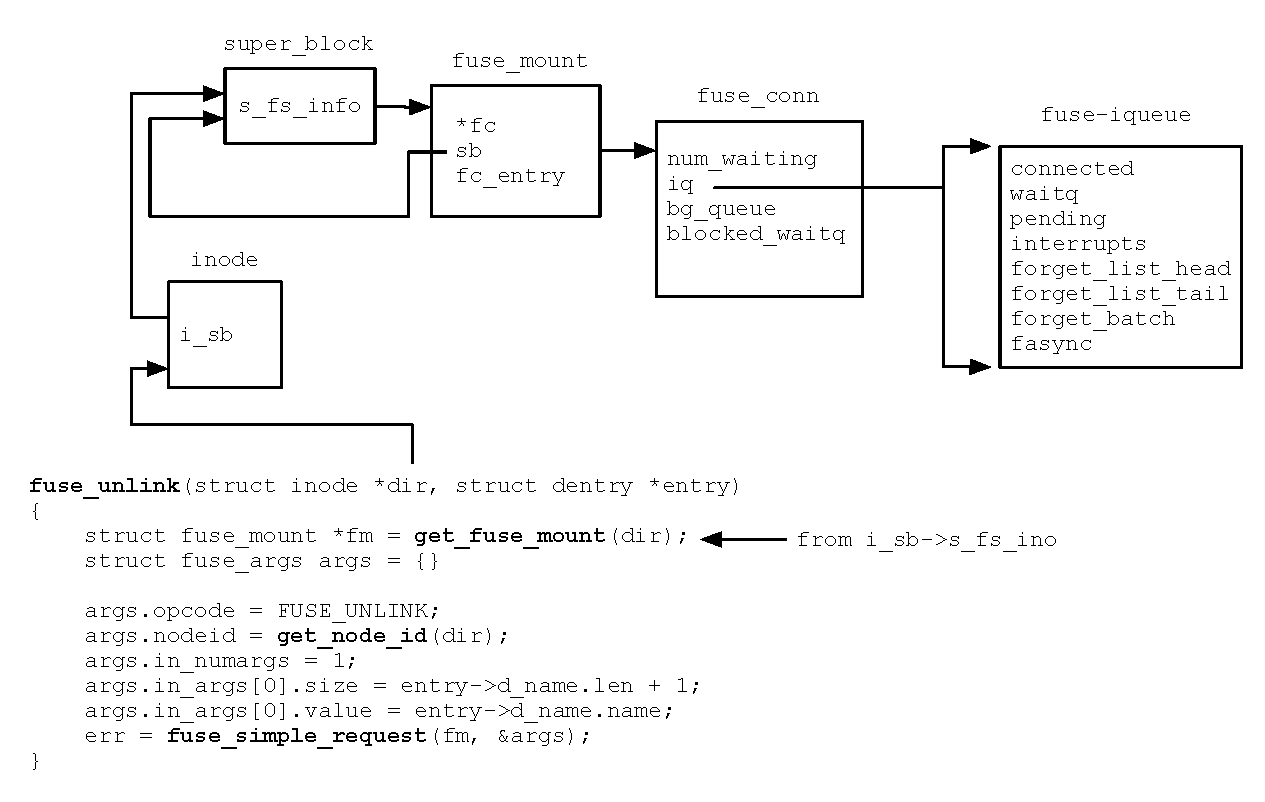
\includegraphics[scale=0.6]{figures/fuse-structs.pdf}
	\centering
	\caption{Structures accessed during most FUSE file operations}
	\label{fig:fuse-structs}
\end{figure}

The unlink request enters the \cf{fuse} filesystem through \cf{fuse\_unlink()} which creates a \cf{FUSE\_UNLINK} request message and calls \cf{fuse\_simple\_request()} to add the message to the list of pending messages. This queue is referenced by the \cf{pending} field of the \cf{fuse\_iqueue} structure. This structure is accessed through the list of structures shown in the figure. The following sections will described these structures in more detail. 

The \cf{libfuse} daemon will read from \cf{/dev/fuse} and should be waiting for messages from the kernel unless it is already processing existing messages. Once a message is posted, the read will complete and the daemon will process the request by calling into the user-space filesystem through the supplied operations vector.

%%%%%%%%%%%%%%%%%%%%%%%%%%%%%%%%%%%%%%%%%%%%%%%%%%%%%%%%%%%%

\section{Digging Under The Covers}

There are just over 16,000 LOC in the FUSE kernel components split across the following source files in \cf{/home/spate/linux-5.19.17/fs/fuse}:

\begin{lstlisting}
$ [*\bfseries ls*]
Kconfig    control.c	dev.c	  fuse_i.h   readdir.c
Makefile   cuse.c       dir.c     inode.c    virtio_fs.c
acl.c      dax.c        file.c    ioctl.c    xattr.c
\end{lstlisting}

\noindent
and one header file \cf{include/linux/uapi/linux/fuse.h} which defines the kernel interface of FUSE. Overall, FUSE doesn't have a huge code base but like many Linux kernel components, it hasn't been well documented.

%%%%%%%%%%%%%%%%%%%%%%%%%%%%%%%%%%%%%%%%%%%%%%%%%%%%%%%%%%%%%%

\subsection{FUSE Kernel Startup}

Figure \ref{fig:fuse-startup} shows the steps performed by \cf{fuse\_init()} from when the FuSE module is first loaded and the module initialization routine (\cf{module\_init(fuse\_init)}) is called. This can be found in \cf{fs/fuse/inode.c}.

\begin{figure}[h]
	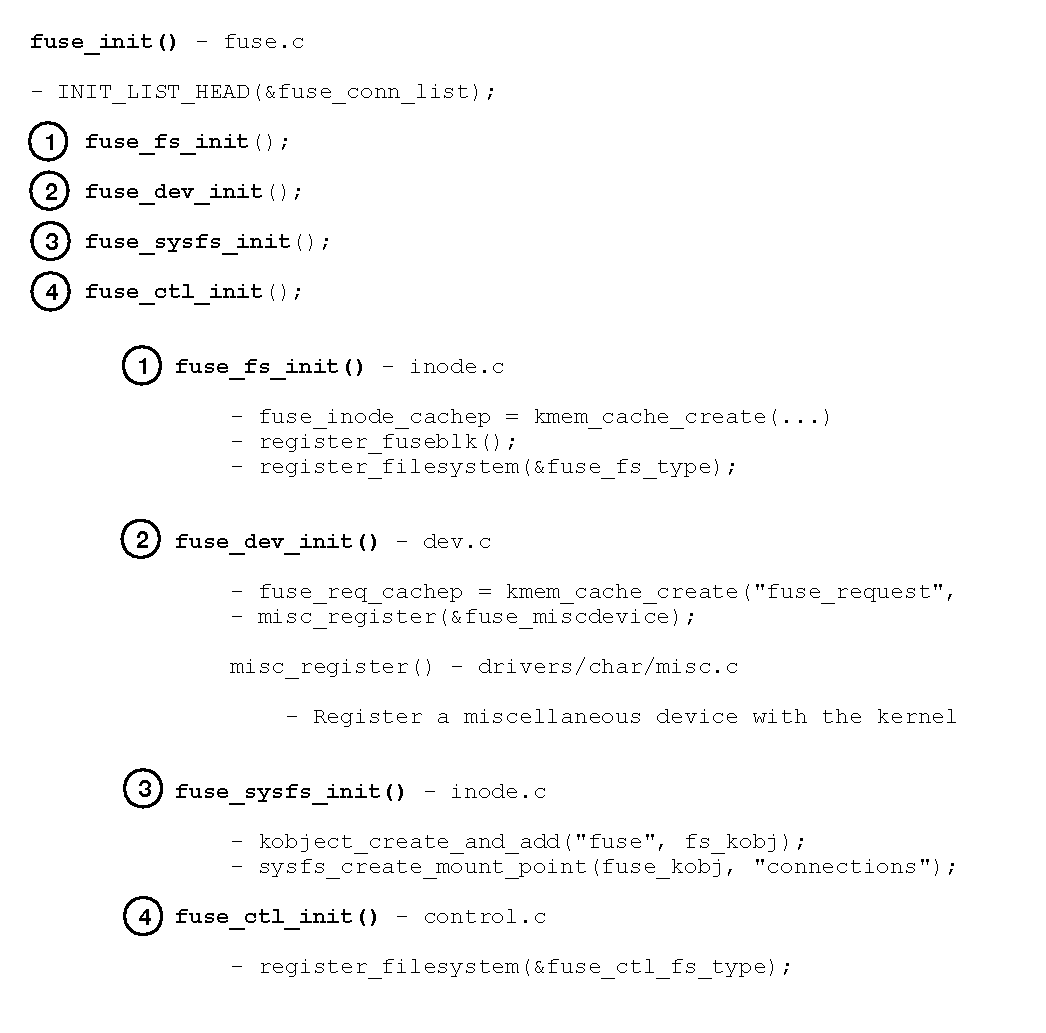
\includegraphics[scale=0.6]{figures/fuse-startup.pdf}
	\centering
	\caption{FUSE Kernel Startup}
	\label{fig:fuse-startup}
\end{figure}

\noindent
The four functions performed during this phase are:

\begin{enumerate}
	\item \cf{fuse\_fs\_init()} -- this call initializes the \cf{fuse} filesystem which is the first entry point into FUSE when
		file requests enter the kernel through the mount point. It also registers the \cf{fuseblk} filesystem. 
		\textbf{XXX---more when understood}.
	\item \cf{fuse\_dev\_init()} -- the character device driver \cf{/dev/fuse} is registered with the kernel through the
		call to \cf{misc\_register()}.
	\item \cf{fuse\_sysfs\_init()} -- this allows all connections (FUSE-mounted filesystems) to be visible through
		\cf{/sys/fs/fuse/connections}.
	\item \cf{fuse\_ctl\_init()} -- this registers the \cf{fusectl} filesystem which allows control and monitoring of  
		FUSE file system behavior.
\end{enumerate}

\noindent
After \cf{fuse\_init()} has completed there are two filesystems (\cf{fuse} and \cf{fusectl}) and one device driver (also called \cf{fuse}) that share code in the same kernel module. 

%%%%%%%%%%%%%%%%%%%%%%%%%%%%%%%%%%%%%%%%%%%%%%%%%%%%%%%%%%%%

\subsection{Establishing Connection between the Kernel and \cf{libfuse}}

Section \ref{pspfs}, describes the pSPFS filesystem, and is the first of three example FUSE filesystems in this chapter showing a passthrough filesystem where operations are passed through a FUSE mount point, through the\cf{libfuse} library and into pSPFS. Here is an abbreviated example of how this filesystem daemon startups up. It declares a list of filesystem operations that it supports and calls into \cf{fuse\_main()} passing this operations vector together with any arguments passed on the command line (including mount point and target filesystem).

\begin{lstlisting}
static struct fuse_operations spfs_operations = {
    .create         = sp_create,
    .unlink         = sp_unlink,
      ...
    .statfs         = sp_statfs
};

int
main(int argc, char *argv[])
{         
    return [*\bfseries fuse\_main*](argc, argv, &spfs_operations, NULL);
}   
\end{lstlisting}

\noindent
When the \cf{libfuse} daemon starts there are several things operations that are performed before the user-space filesystem can be accessed.  Note that two functions described are defined as macros in \cf{include/fuse.h}:

\begin{itemize}
	\item \cf{fuse\_main} is defined as \cf{fuse\_main\_real}. 
	\item \cf{fuse\_new} is defined as \cf{fuse\_new\_31}. 
\end{itemize}

\noindent	
You can find \cf{fuse\_main\_real()} in the \cf{lib} directory. Note that the following text will still use the function names \cf{fuse\_main()} and \cf{fuse\_new}. There is a useful comment above the macro definition in this header file that describes the process followed by \cf{fuse\_main()} and error codes that can be returned.

The steps followed by \cf{fuse\_main()} are as follows and shown in figure \ref{fig:libfuse-path-and-structs}. All functions in the \cf{libfuse} library described can be found under the \cf{lib} directory.

\begin{enumerate}
	\item pSPFS calls \cf{fuse\_main()} which parses the arguments 
		passed to the program by calling \cf{fuse\_parse\_cmdline()}. It then calls \cf{fuse\_mount()}.
	\item \cf{fuse\_mount()} creates a UNIX domain socket pair, then forks and executes the 
		\cf{fusermount(1)} command (\cf{util/fusermount.c}) passing it one end of the socket.
	\item \cf{fusermount()} makes sure that the FUSE module is loaded then opens \cf{/dev/fuse} 
		and sends the file handle back to \cf{fuse\_mount()}.
	\item \cf{fuse\_mount()} returns the file handle for \cf{/dev/fuse} to \cf{fuse\_main()}.
	\item \cf{fuse\_main()} calls \cf{fuse\_new()} (in \cf{lib/fuse.c}) to allocate a '\cf{struct fuse}' object that stores 
		and maintains a cached image of the filesystem data. \textbf{XXX---what cached image?}
	\item \cf{fuse\_main()} calls either \cf{ fuse\_loop()} or \cf{fuse\_loop\_mt()} 
		which starts to read the filesystem system calls from \cf{/dev/fuse}, call the user-supplied  functions stored in a 
		'\cf{struct fuse\_operations}' object before calling \cf{fuse\_main()}.  The results of those calls are then written 
		back to the \cf{/dev/fuse} file where they can be forwarded back through the \cf{fuse} filesystem and allow
		thesystem calls to return.
\end{enumerate}

\noindent
The figure shows the structures that are allocated prior to entering \cf{fuse\_loop()} or \cf{fuse\_look\_mt\_32()}. From here you can see the file descriptor that is use to access \cf{/dev/fuse} as well as the low-level and high-level operations vectors that the user-space filesystem provided when calling \cf{fuse\_main()}.

\begin{figure}[h]
	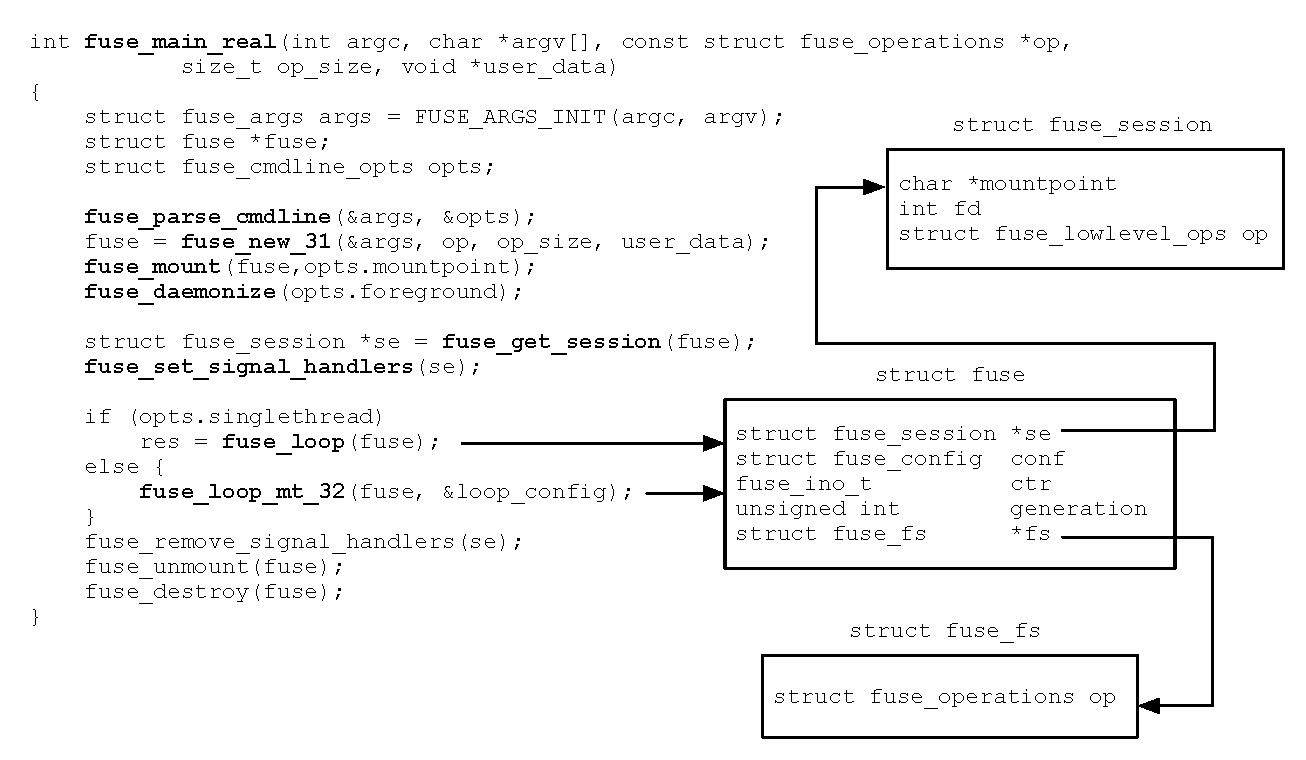
\includegraphics[scale=0.6]{figures/libfuse-path-and-structs.pdf}
	\centering
	\caption{Startup paths for \cf{libfuse}}
	\label{fig:libfuse-path-and-structs}
\end{figure}

\noindent
The \cf{fuse\_loop()} function calls \cf{fuse\_session\_loop()} which sits in a loop as the following fragment of code shows:

\begin{lstlisting}
int fuse_session_loop(struct fuse_session *se)
{
    while (!fuse_session_exited(se)) {
        res = fuse_session_receive_buf_int(se, &fbuf, NULL);
        fuse_session_process_buf_int(se, &fbuf, NULL); 
    }
}
\end{lstlisting}

\noindent
\textbf{XXX---where does struct fuse / fuse\_fs go? The latter has the ops vector}



%%%%%%%%%%%%%%%%%%%%%%%%%%%%%%%%%%%%%%%%%%%%%%%%%%%%%%%%%%%%%%%%
\subsection{Mounting a \cf{fuse} Filesystem}

XXX - should cover fusemount since that's what kicks it off

XXX - cover INIT - when fs is being mounted see one 2. DESTROY sent when fs is unmounted and there will be no more kernel requests. probably new section for latter

\textbf{XXX---not sure this is the right place but will see}

When most filesystems register they declare a \textit{mount} function as part of the \cf{file\_system\_type} structure which is passed to \cf{register\_filesystem()}. The \cf{fuse} filesystem does not register such a function. There is a fn \cf{fuse\_fill\_super()} in the kernel but can't see who calls it.

\begin{lstlisting}
https://docs.kernel.org/filesystems/mount_api.html - 
describes a newer mount process. Looks like a lot of 
filesystems are doing this now so might want to switch SPFS too?

NOTE - see fs/fs_context.c for how this function is handled

The creation of new mounts is now to be done in a multistep process:

1. Create a filesystem context.
2. Parse the parameters and attach them to the context. Parameters 
are expected to be passed individually from userspace, though legacy 
binary parameters can also be handled.
3. Validate and pre-process the context.
4. Get or create a superblock and mountable root.
5. Perform the mount.
6. Return an error message attached to the context.
7. Destroy the context.

To support this, the file_system_type struct gains two new fields:

int (*init_fs_context)(struct fs_context *fc);
const struct fs_parameter_description *parameters;
\end{lstlisting}

\noindent
Let's go explore this some more. The \cf{fuse} filesystem declares \cf{fuse\_init\_fs\_context()} and here it is:

\begin{lstlisting}
static int fuse_init_fs_context(struct fs_context *fsc)
{
    struct fuse_fs_context *ctx;

    ctx = kzalloc(sizeof(struct fuse_fs_context), GFP_KERNEL);

    ctx->max_read = ~0;
    ctx->blksize = FUSE_DEFAULT_BLKSIZE;
    ctx->legacy_opts_show = true;

    fsc->fs_private = ctx;
    fsc->ops = &fuse_context_ops;
    return 0;
}

static const struct fs_context_operations fuse_context_ops = {
    .free       = fuse_free_fsc,
    .parse_param    = fuse_parse_param,
    .reconfigure    = fuse_reconfigure,
    .get_tree   = fuse_get_tree,
};
\end{lstlisting}

\noindent
xxx

%%%%%%%%%%%%%%%%%%%%%%%%%%%%%%%%%%%%%%%%%%%%%%%%%%%%%%%%%%%%%%%%

\subsection{General Flow Between Kernel and User-space}\label{general-flow}

The kernel doc has a nice example of the flow between the kernel and \cf{libfuse} in response to an \cf{unlink(2)} system call. Figure \ref{fig:fuse-flow-to-daemon} gives an expanded version and brings it more up to date with the existing FUSE code base. The angle brackets show when a function is entered and when it exits. For example, \cf{> sys\_read()} shows the function being entered and 

Can really put a pause in the daemon and see the kernel stack from the requesting process \cf{< sys\_read()} shows when it exits.

\textbf{unused\_list - doesn't exist in the source code so need to figure out what's correct}

\begin{figure}
	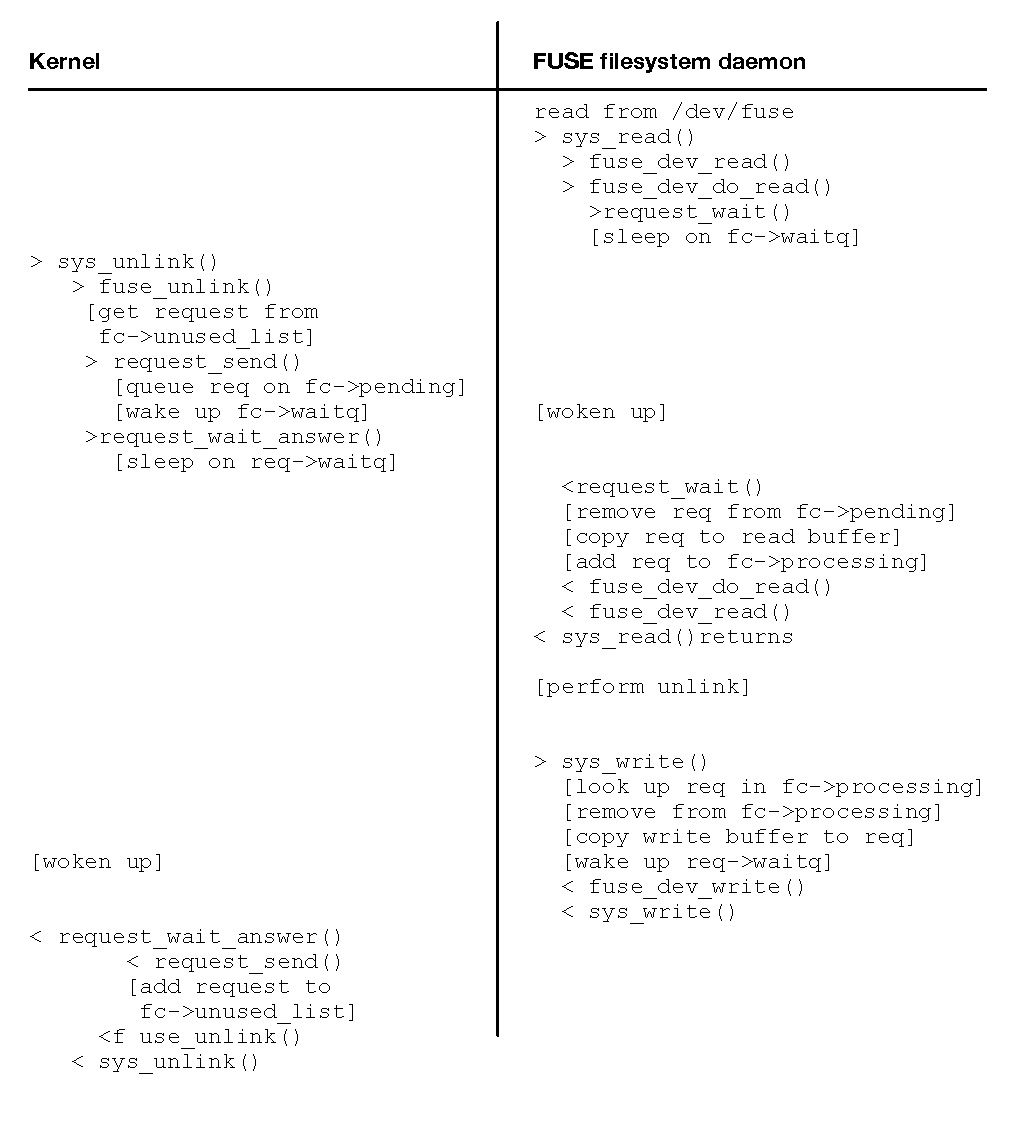
\includegraphics[scale=0.7]{figures/fuse-flow-to-daemon.pdf}
	\centering
	\caption{Flow between the kernel and the FUSE daemon}
	\label{fig:fuse-flow-to-daemon}
\end{figure}

\noindent
xxx

%%%%%%%%%%%%%%%%%%%%%%%%%%%%%%%%%%%%%%%%%%%%%%%%%%%%%%%%%%%%%%%%

\subsection{FUSE VFS Interfaces}

The \cf{fuse} kernel filesystem provides the following operations vectors. These vectors are defined in \cf{fs/fuse/dir.c} and \cf{fs/fuse/file.c}

\begin{lstlisting}
struct super_operations         fuse_super_operations
struct export_operations        fuse_export_operations

struct inode_operations         fuse_dir_inode_operations
struct inode_operations         fuse_common_inode_operations
struct inode_operations         fuse_symlink_inode_operations 
struct file_operations          fuse_dir_operations
struct address_space_operations fuse_file_aops
\end{lstlisting}

\noindent
The first two vectors deal with filesystem-related operations. The first is attached to the \cf{s\_op} and \cf{s\_export\_op} fields of the \cf{super\_block} structure respectively. The other five vectors are attached to the \cf{i\_op} or \cf{i\_fop} and \cf{i\_data.a\_ops} fields of the \cf{inode} structure depending on the vector and the file type.

Each \cf{fuse} filesystem VFS entry point follows a similar path. Take \cf{fuse\_mkdir()} as an example and also compare with a very similar path taken by \cf{fuse\_unlink()} (figure \ref{fig:fuse-structs}). A message is created with the appropriate arguments needed for the \cf{libfuse} daemon to fulfill the request, the message is queued and if the daemon is waiting for a request, it will be woken up.

\begin{lstlisting}
static int fuse_rmdir(struct inode *dir, struct dentry *entry)
{
    int err;
    struct fuse_mount *fm = [*\bfseries get\_fuse\_mount(dir)*];
    FUSE_ARGS(args);  /* struct fuse_args */

    /* Fill in fuse_args with information needed by libfuse 
       and the user-space filesystem */
    
    args.opcode = FUSE_RMDIR;
    args.nodeid = get_node_id(dir);
    args.in_numargs = 1;
    args.in_args[0].size = entry->d_name.len + 1;
    args.in_args[0].value = entry->d_name.name;
    
    /* Add the message to the pending list*/
    
    err = [*\bfseries fuse\_simple\_request(fm, \&args)*];

    if (!err) {
        fuse_dir_changed(dir);
        fuse_entry_unlinked(entry);
    }
    return err;
}
\end{lstlisting}

\noindent
A call to \cf{get\_node\_id()} gets the \cf{fuse} inode (of type \cf{struct fuse\_inode}) and returns the \cf{nodeid} field. This is a Unique ID, which identifies the inode between user-space and kernel. \textbf{XXX---it must be the inode number returned by the FUSE daemon otherwise what else would it be? It's passed as an argument so look some more at the inode/daemon code}.

A call to \cf{get\_fuse\_mount()} returns the \cf{fuse\_mount} structure that is referenced from the \cf{s\_fs\_info} field of the \cf{super\_block} structure for this mount point. 

The \cf{struct fuse\_args} structure is defined in \cf{fuse/fuse\_i.h}. Here is a subset of the structure:

\begin{lstlisting}
struct fuse_args {
    uint64_t nodeid;
    uint32_t opcode;
    unsigned short in_numargs;
    unsigned short out_numargs;
    ...
    struct fuse_in_arg in_args[3];
    struct fuse_arg out_args[2];
    void (*end)(struct fuse_mount *fm, struct fuse_args *args, 
                int error);
};
\end{lstlisting}

\noindent
The \cf{opcode} field represents the operation that is performed by the user-space filesystem. In the \cf{libfuse} source code, the \cf{fuse\_ll\_ops} structure (\cf{fuse\_lowlevel.c}) contains all of the opcodes and functions that will be called. For example, for \cf{FUSE\_RMDIR}, a call will be made to \cf{do\_rmdir()}: 

\begin{lstlisting}
static void do_rmdir(fuse_req_t req, fuse_ino_t nodeid, 
                     const void *inarg)
{   
    char *name = (char *) inarg;       
    
    if (req->se->op.rmdir) 
        [*\bfseries req->se->op.rmdir(req, nodeid, name);*]
    else
        fuse_reply_err(req, ENOSYS);       
}   
\end{lstlisting}

\noindent
The \cf{rmdir} function called here is the function provided by the user-space filesystem.

%%%%%%%%%%%%%%%%%%%%%%%%%%%%%%%%%%%%%%%%%%%%%%%%%%%%%%%%%%%%%%%%

\subsection{FUSE to \cf{libfuse} Request Queues}

There are five FUSE queues that are used to communicate between the \cf{fuse} filesystem and \cf{libfuse} through the \cf{fuse} device driver. These queues are:

\begin{enumerate}
	\item \textbf{pending} -- for synchronous requests - looks like FUSE calls this the input queue (see definition of 
		\cf{fuse\_conn}, element \cf{iq})
	\item \textbf{background} -- for async requests??? 
	\item \textbf{processing} -- when a message has been picked up for processing it is moved from the pending queue
		to the processing queue. XXX - Same for others????
	\item \textbf{forgets} -- not related to above (requests posted here separately)
	\item \textbf{interrupts} -- not related to above (requests posted here separately)
\end{enumerate}

\noindent
Some are initialized in \cf{fuse\_iqueue\_init()} which is passed a \cf{fuse\_iqueue} structure.

\cf{fuse\_get\_tree} -> \cf{fuse\_conn\_init()} -> \cf{fuse\_iqueue\_init()} - first function called during mount processing and also described elsewhere here.

\begin{lstlisting}
static void fuse_iqueue_init(struct fuse_iqueue *fiq,
                 const struct fuse_iqueue_ops *ops,
                 void *priv)
{
    memset(fiq, 0, sizeof(struct fuse_iqueue));
    spin_lock_init(&fiq->lock);
    init_waitqueue_head(&fiq->waitq);
    INIT_LIST_HEAD(&fiq->pending);
    INIT_LIST_HEAD(&fiq->interrupts);
    fiq->forget_list_tail = &fiq->forget_list_head;
    fiq->connected = 1;
} 
\end{lstlisting}

\noindent
Here are the relevant fields in the \cf{fuse\_iqueue} structure:

\begin{lstlisting}
struct fuse_iqueue {
    struct list_head         [*\bfseries pending;*]
    struct list_head         [*\bfseries interrupts;*]
    struct fuse_forget_link  [*\bfseries forget\_list\_head;*]
    struct fasync_struct    *[*\bfseries fasync;*]
}
\end{lstlisting}

\noindent
The \textit{processing queue} is inside the \cf{fuse\_dev} structure as follows: \textbf{XXX - but where is this bugger?}

\begin{lstlisting}
struct fuse_dev {
    struct fuse_conn   *fc;    /* Fuse connection for this dev */
    struct fuse_pqueue  [*\bfseries pq;*]    /* Processing queue */
    struct list_head    entry; /* list entry on fc->devices */
};
\end{lstlisting}

\noindent
It's not obvious who sets file->private\_data as it's set to NULL in open below and then assumed to be there when reading /dev/fuse. it's set by \cf{fuse\_do\_open()} but who calls this?

\begin{lstlisting}
static int fuse_dev_open(struct inode *inode, struct file *file)
{
    /*
     * The fuse device's file's private_data is used to hold
     * the fuse_conn(ection) when it is mounted, and is used to
     * keep track of whether the file has been mounted already.
     */
    file->private_data = NULL;
    return 0;
}

static ssize_t 
fuse_dev_read(struct kiocb *iocb, struct iov_iter *to)
{
    struct file *file = iocb->ki_filp;
    struct fuse_dev *fud = fuse_get_dev(file);  

    return fuse_dev_do_read(fud, file, &cs, iov_iter_count(to));
}

static ssize_t 
fuse_dev_do_read(struct fuse_dev *fud, struct file *file,
                 struct fuse_copy_state *cs, size_t nbytes)
{
    struct fuse_pqueue *fpq = &fud->pq;
}
\end{lstlisting}

\noindent
\cf{fuse\_get\_tree()} calls \cf{fuse\_conn\_init()} which calls \cf{fuse\_iqueue\_init()}

\noindent
Requests are zzz the \cf{fuse\_req} structure which can be found in \cf{fs/fuse/fuse\_i.h}

\begin{lstlisting}
struct fuse_req {
    struct list_head list;
    struct list_head intr_entry;
    struct fuse_args *args;
    refcount_t count;
    unsigned long flags;
    struct {
        struct fuse_in_header h; /* The request input header */
    } in;
    struct {
        struct fuse_out_header h; /* The request output header */
    } out;
    wait_queue_head_t waitq;
    void *argbuf;
    struct fuse_mount *fm; /** fuse_mount this request belongs to */
};
\end{lstlisting}

\noindent
xxx

\begin{lstlisting}
fuse_request_alloc() -> kmem_cache_zalloc()
\end{lstlisting}

\noindent
As described earlier, the \cf{fuse} filesystem operations for many regular file operations involves creating a message containing all the information needed to process the request in the \cf{libfuse} daemon and then make a call to \cf{fuse\_simple\_request()} to queue the request.

\begin{lstlisting}
ssize_t fuse_simple_request(struct fuse_mount *fm, 
                            struct fuse_args *args)
{
    req = fuse_request_alloc(fm, GFP_KERNEL | __GFP_NOFAIL);
or
    req = fuse_get_req(fm, false);
 
     __fuse_request_send(req);
}

static void __fuse_request_send(struct fuse_req *req)
{
    struct fuse_iqueue *fiq = &req->fm->fc->iq;

    __fuse_get_request(req);
    queue_request_and_unlock(fiq, req);
}
\end{lstlisting}

\noindent
XXX and then adds the message to the tail end of the \textit{pending} queue as follows:

\begin{lstlisting}
static void queue_request_and_unlock(struct fuse_iqueue *fiq,
                     struct fuse_req *req)
{
    req->in.h.len = sizeof(struct fuse_in_header) +
        fuse_len_args(req->args->in_numargs,
                  (struct fuse_arg *) req->args->in_args);
    list_add_tail(&req->list, &fiq->pending);
    fiq->ops->wake_pending_and_unlock(fiq);
}
\end{lstlisting}

\noindent
xxx

\begin{lstlisting}
static void fuse_dev_wake_and_unlock(struct fuse_iqueue *fiq)
{
    wake_up(&fiq->waitq);
    kill_fasync(&fiq->fasync, SIGIO, POLL_IN);
    spin_unlock(&fiq->lock);
}
\end{lstlisting}

\noindent
xxx

%%%%%%%%%%%%%%%%%%%%%%%%%%%%%%%%%%%%%%%%%%%%%%%%%%%%%%%%%%%%%%%%

\subsection{Kernel to \cf{libfuse} Messages}

In the \cf{fuse.h} header file, "\cf{enum fuse\_opcode}" defines all of the kernel to \cf{libfuse} message types that both sides used during communication. Several of them are also described in the \cf{fuse(4)} manpage.

\begin{lstlisting}
enum fuse_opcode {
    FUSE_LOOKUP             = 1,
    FUSE_FORGET             = 2,  /* no reply */
    FUSE_GETATTR            = 3,
    FUSE_SETATTR            = 4,
    FUSE_READLINK           = 5,
    FUSE_SYMLINK            = 6,
    ...
    FUSE_REMOVEMAPPING      = 49,
    FUSE_SYNCFS             = 50,
}
\end{lstlisting}

\noindent
For most of these message types, there will be a corresponding \cf{fuse} filesystem VFS function that processes the system call. This was shown earlier but for completeness, here is the \cf{fuse} VFS function supporting the \cf{symlink(2)} system call with the VFS function and opcode highlighted:

\begin{lstlisting}
static int [*\bfseries fuse\_symlink*](struct user_namespace *mnt_userns, 
                        struct inode *dir, struct dentry *entry, 
                        const char *link)
{   
    struct fuse_mount *fm = get_fuse_mount(dir);
    unsigned len = strlen(link) + 1;
    FUSE_ARGS(args);
    
    args.opcode = [*\bfseries FUSE\_SYMLINK*];
    args.in_numargs = 2;
    ...
}   
\end{lstlisting}

\noindent
The message to send to \cf{libfuse} is constructed and put on the pending queue to be picked up by the daemon. In \cf{libfuse} there is a structure in \cf{fuse\_lowlevel.c} called \cf{fuse\_ll\_ops} that contains the same list of opcodes plus all of the functions that are called in response. Here is a fragment showing \cf{FUSE\_SYMLINK}:

\begin{lstlisting}
static struct {
    void (*func)(fuse_req_t, fuse_ino_t, const void *);
    const char *name;
} fuse_ll_ops[] = {
    [FUSE_LOOKUP]      = { do_lookup,    "LOOKUP"      },
    ...
    [[*\bfseries FUSE\_SYMLINK*]]     = { [*\bf do\_symlink*],     "SYMLINK"     },
    ...
}
\end{lstlisting}

\noindent
The \cf{libfuse} functions in this structure follow a similar path in terms of marshaling the arguments and calling the user-level filesystem provided function if one is available. Here is the \cf{do\_symlink} function:

\begin{lstlisting}
static void do_symlink(fuse_req_t req, fuse_ino_t nodeid, 
                       const void *inarg)
{   
    char *name = (char *) inarg;
    char *linkname = ((char *) inarg) + 
                      strlen((char *) inarg) + 1;
    
    if (req->se->op.symlink)
        req->se->op.[*\bfseries symlink*](req, linkname, nodeid, name);
    else
        fuse_reply_err(req, ENOSYS);   
}   
\end{lstlisting}

\noindent
If you look at other functions in \cf{fuse\_lowlevel.c} you will see that they all follow a very similar path.

%%%%%%%%%%%%%%%%%%%%%%%%%%%%%%%%%%%%%%%%%%%%%%%%%%%%%%%%%%%%%%%%

\subsection{Controlling FUSE Through \cf{fusectl}}\label{fusectl}

For each \cf{fuse} mounted filesystem, the \cf{fusectl} filesystem creates a directory named by a unique number that gives information about each mountpoint. \textbf{XXX - find where it is created}

The \cf{fusectl} source code can be found in \cf{fs/fuse/control.c}. Each time a FUSE filesystem is mounted,  \cf{fuse\_fill\_super\_common()} in the \cf{fuse} filesystem will make a call into \cf{fusectl} to create the appropriate tree structure for the new mount point under \cf{/sys/fs/fuse/connections} as follows:

\begin{lstlisting}
fuse_ctl_add_conn() 
{
    sprintf(name, "%u", fc->dev);
    parent = fuse_ctl_add_dentry(parent, fc, name, 
                     S_IFDIR | 0500, 2,
                     &simple_dir_inode_operations,
                     &simple_dir_operations);

    if (!fuse_ctl_add_dentry(parent, fc, "waiting", 
                 S_IFREG | 0400, 1,
                 NULL, &fuse_ctl_waiting_ops) ||
        !fuse_ctl_add_dentry(parent, fc, "abort", 
                 S_IFREG | 0200, 1,
                 NULL, &fuse_ctl_abort_ops) ||
        !fuse_ctl_add_dentry(parent, fc, "max_background", 
                 S_IFREG | 0600,
                 1, NULL, &fuse_conn_max_background_ops) ||
        !fuse_ctl_add_dentry(parent, fc, "congestion_threshold",
                 S_IFREG | 0600, 1, NULL,
                 &fuse_conn_congestion_threshold_ops))
    ...
}
\end{lstlisting}

\noindent
For each connection the following files exist within this directory:

\begin{itemize}
	\item \cf{waiting} -- the number of requests which are waiting to be transferred to user-space or being processed by the
		FUSE filesystem daemon.  If there is no filesystem activity and \cf{waiting} is non-zero, the filesystem is hung 
		or deadlocked.
	\item \cf{abort} -- writing anything into this file will abort the filesystem connection. All requests waiting will be aborted and 
		an error returned for all aborted and new requests.
	\item \cf{congestion\_threshold} -- if the number of outstanding requests exceeds the value visible in this file (9 by default
	 	and 75\% of \cf{max\_background}, the filesystem will be marked as "congested". 
		This changes the way in which FUSE components handle subsequent requests assuming that the filesystem 
		daemon will take some time to complete requests. One such action is to sleep rather than waiting in a busy loop.
	\item \cf{max\_background} -- requests in the background (async) queue move to the pending queue over time. This
		value defines the limit of such requests that can reside on the pending queue in order to prevent synchronous
		requests from being delayed significantly - \textbf{XXX---the ACM doc has good info so come back to this
		once i do the performance section}
\end{itemize}

\noindent
Only the owner of the mount may read or write these files.

\begin{lstlisting}
$ [*\bfseries ls /sys/fs/fuse/connections/*]
47/
$ [*\bfseries ls /sys/fs/fuse/connections/47*]
abort  congestion_threshold  max_background  waiting
\end{lstlisting}

\noindent
\textbf{XXX---i'm going to do an example where an op goes to sleep so i can look at stack traces etc. come back and show \cf{waiting} which should go to "1"}

%%%%%%%%%%%%%%%%%%%%%%%%%%%%%%%%%%%%%%%%%%%%%%%%%%%%%%%%%%%%%%

\subsection{Multithreading}

I guess mostly in the library? \textbf{this is all copied from the web}

\begin{quote}
Background: When a file is opened, the Linux kernel creates a "file description" for the I/O state, and returns a "file descriptor" to userland. That descriptor can be freely passed to the dup(2) functions to duplicate the descriptor, but the underlying description remains unary.

The FUSE kernel driver implicitly locks access to the /dev/fuse file descriptor so that each read() and write() syscall is atomic. This implies that multiple threads can safely share the descriptor, but also that they will face lock contention and reduced performance.

To get the best performance out of a multi-threaded filesystem server, open /dev/fuse once as a "session FD" and again in each thread as "worker FDs". After initializing the session with a standard FUSE handshake, the workers can be associated with the session by calling ioctl(worker\_fd, FUSE\_DEV\_IOC\_CLONE, \&session\_fd).

This allows multiple threads to serve FUSE requests without contending for the descriptor lock.
\end{quote}

%%%%%%%%%%%%%%%%%%%%%%%%%%%%%%%%%%%%%%%%%%%%%%%%%%%%%%%%%%%%%%

\subsection{Time to FORGET}

Cover FORGET. Daemon May cache a lot of stuff rather than my simple pass trough so important - this is from the ACM paper

\begin{quote}
Every time an existing inode is looked up (or a new one is created), the kernel keeps the inode in the inode and directory entry cache (dcache). When removing an inode from the dcache, the kernel passes the FORGET request to the FUSE daemon. FUSE's inode reference count (in user-space file systems) grows by one with every reply to LOOKUP, CREATE, and so forth, requests. FORGET requests pass an nlookups parameter which informs the user-space file system (the FUSE daemon) how many lookups to forget. At this point, the user-space file system (the FUSE daemon) might decide to deallocate any corresponding data structures (once their reference count goes to 0). BATCH\_FORGET allows the kernel to forget multiple inodes with a single request.
\end{quote}

%%%%%%%%%%%%%%%%%%%%%%%%%%%%%%%%%%%%%%%%%%%%%%%%%%%%%%%%%%%%%%

\subsection{FUSE Interrupts}

\textbf{taken from web so rewrite}

If a process issuing a FUSE filesystem request is interrupted, the following happens:

1) if the request is not yet sent to user-space AND the signal is fatal, the request is dequeued and returns immediately.

2) if the request is not yet sent to user-space AND the signal is not fatal, an 'interrupted' flag is set for the request.  When the request has been successfully transferred to user-space and this flag is set, an INTERRUPT request is queued.

3) if the request is already sent to user-space, then an INTERRUPT request is queued.

INTERRUPT requests take precedence over other requests, so the user-space filesystem receives queued INTERRUPTs before any others.

The user-space filesystem may ignore the INTERRUPT requests entirely, or may honor them by sending a reply to the "original" request, with the error set to EINTR (the call did not succeed because it was interrupted)

It is also possible that there is a race between processing the original request and it's INTERRUPT request.  There are two possibilities:

1) The INTERRUPT request is processed before the original request is processed

2) The INTERRUPT request is processed after the original request has been answered

If the filesystem cannot find the original request, it should wait for some timeout and/or a number of new requests to arrive, after which it should reply to the INTERRUPT request with an EAGAIN error.  In case

1) the INTERRUPT request will be re-queued.  In case 2) the INTERRUPT reply will be ignored.

The \cf{fuse\_read\_interrupt()} function sends a message of type \cf{FUSE\_INTERRUPT}. \textbf{XXX---hmm need to look more at this}

%%%%%%%%%%%%%%%%%%%%%%%%%%%%%%%%%%%%%%%%%%%%%%%%%%%%%%%%%%%%%%%%

\subsection{Per-File DAX Option}

% https://www.phoronix.com/news/Linux-5.17-FUSE-Per-inode-DAX

TBD - per-file direct access (DAX) - just something else to look at

%%%%%%%%%%%%%%%%%%%%%%%%%%%%%%%%%%%%%%%%%%%%%%%%%%%%%%%%%%%%%%%%

\subsection{The \cf{fuseblk} Filesystem}

might help - % https://linuxhint.com/use-fuseblk-linux/ 
and % https://unix.stackexchange.com/questions/332712/how-do-i-find-out-what-filesystem-fuse-is-using

One area that has little documentation is around \cf{fuseblk} for which the target is block device and not a filesystem or a directory within an existing filesystem. There has been little usage of\cf{fuseblk} although the most common usage that has been described on the web is for supporting NTFS-3G, a FUSE-based NTFS filesystem that was introduced in 2007. The developers of NTFS-3G later formed Tuxera Inc., producing Tuxera NTFS, a proprietary version. NTFS-3G is now the free "community edition".

In 2021, a different version of NTFS was merged into the mainline kernel. Linux Torvalds complained about the performance of NTFS-3G. Can you read about the discussions/arguments around this choice here:

\begin{table}[h]
\begin{tabular}{lcl}
\parbox[r]{0.5in}{
\includegraphics[scale=0.15]{figures/url.png}} & \parbox[l]{0.55in}{URL \arabic{urls} -- } & \parbox[l]{3in}{\cf{https://tinyurl.com/yvnmc5bp}}
\end{tabular}
\end{table}
\stepcounter{urls}
% https://www.theregister.com/2021/10/13/how_ntfs_finally_made_it/

\noindent
xxx - code is in fuse/inode.c for registering the filesystem There is also fuse/dev.c

\begin{lstlisting}
static struct file_system_type fuseblk_fs_type = {
    .owner           = THIS_MODULE,
    .name            = "fuseblk",
    .init_fs_context = fuse_init_fs_context,
    .parameters      = fuse_fs_parameters,
    .kill_sb         = fuse_kill_sb_blk,
    .fs_flags        = FS_REQUIRES_DEV | FS_HAS_SUBTYPE,
};  
MODULE_ALIAS_FS("fuseblk");

static inline int register_fuseblk(void)
{
    return register_filesystem(&fuseblk_fs_type);
}   
    
static inline void unregister_fuseblk(void)
{   
    unregister_filesystem(&fuseblk_fs_type);
} 
\end{lstlisting}

\noindent
Note that there is no mount function declared as per SPFS et al so why a filesystem type?

Examples

NTFS - % https://linuxhint.com/use-fuseblk-linux/
NTFS-3G - https://en.wikipedia.org/wiki/NTFS-3G
% https://unix.stackexchange.com/questions/463051/stat-f-says-type-fuseblk-it-should-be-type-fuse

%%%%%%%%%%%%%%%%%%%%%%%%%%%%%%%%%%%%%%%%%%%%%%%%%%%%%%%%%%%%%%%%

\subsection{FUSE and Fsnotify}

article about FUSE and fsnotify which dates back to 2016 and says that fsnotify doesn't work - take a look % https://github.com/libfuse/libfuse/wiki/Fsnotify-and-FUSE 

%%%%%%%%%%%%%%%%%%%%%%%%%%%%%%%%%%%%%%%%%%%%%%%%%%%%%%%%%%%%%%%%

\subsection{User-space Character Devices}

TBD

%%%%%%%%%%%%%%%%%%%%%%%%%%%%%%%%%%%%%%%%%%%%%%%%%%%%%%%%%%%%%%%%

\section{More on \cf{libfuse}}

XXX - needed or not? could add earlier

%%%%%%%%%%%%%%%%%%%%%%%%%%%%%%%%%%%%%%%%%%%%%%%%%%%%%%%%%%%%%%%%

\subsection{The \cf{fuse\_file\_info} Structure}

For all operations in the low-level (or high-level?) API, a \cf{fuse\_file\_info} structure is passed as an argument. This structure is passed between the kernel and \cf{libfuse} for open instances of a file.

This structure is only in \cf{fuselib} and not in the kernel so the library must construct it from whatever messages it receives from the kernel.

\begin{lstlisting}
struct fuse_file_info {
    int           flags; 
    int           writepage; 
    unsigned int  direct_io : 1;
    unsigned int  keep_cache : 1;
    unsigned int  flush : 1;
    unsigned int  nonseekable : 1;
    unsigned int  flock_release : 1;
    uint64_t      fh; 
    uint64_t      lock_owner;
};
\end{lstlisting}

\noindent
The \cf{fh} field is a \cf{file handle} set by a FUSE daemon during an open call to store the file descriptor returned by \cf{open(2)}. When passed to the daemon in subsequent calls (say read and write), the daemon can make system calls using this file handle and avoid having to open the file on each call. This has obvious performance advantages. 

\textbf{XXX---need to see what other fields are worth describing. Who uses them?}

%%%%%%%%%%%%%%%%%%%%%%%%%%%%%%%%%%%%%%%%%%%%%%%%%%%%%%%%%%%%%%

\section{Implementing a FUSE-based Filesystem}\label{pspfs}

This section presents three different FUSE-based filesystems. The most simple filesystem called pSPFS ("p" for passthrough) is only 232 lines of code (including a lot of logging) so is very simple to understand. A modified version called eSPFS is a little more complicated since it provides encryption/decryption of regular file contents. Both of these filesystems use the high-level FUSE APIs. A third example explores one of the \cf{libfuse} example filesystems which provides a single file which shows the current time each time the file is read.

All code can be found here - \textbf{github-XXX}

%%%%%%%%%%%%%%%%%%%%%%%%%%%%%%%%%%%%%%%%%%%%%%%%%%%%%%%%%%%%%%%%

\subsection{Installing FUSE and Compiling the Filesystem}

To use an existing FUSE filesystem requires XXX - \textbf{XXX---redo all of this. it's not just to use and existing FS. libfuse-dev is needed to build daemons. Divide into what's needed to say 1) use SSHFS and 2) build pSPFS}

On Ubuntu it's as simple as:

\begin{lstlisting}
$ [*\bfseries sudo apt-get update -y*]
$ [*\bfseries sudo apt install fuse*]
$ [*\bfseries sudo apt install libfuse-dev*]
$ [*\bfseries sudo apt install pkg-config*]
\end{lstlisting}

\noindent
or do I need to install fuse3?

%%%%%%%%%%%%%%%%%%%%%%%%%%%%%%%%%%%%%%%%%%%%%%%%%%%%%%%%%%%%%%%%

\subsection{Getting Started}

First we need to determine what operations we will support. The full list can be found in \cf{fuse.h} and there are 50 functions that a FUSE daemon can support at the time of writing. Here are the operations that pSPFS supports (11 in total). It's interesting to know which functions to support. For example, I didn't have anything for \cf{utimens} but then saw an error when running \cf{touch file}.

\begin{lstlisting}
static struct fuse_operations spfs_operations = {
    .create         = sp_create,
    .unlink         = sp_unlink,
    .open           = sp_open,
    .read           = sp_read,
    .write          = sp_write,
    .getattr        = sp_getattr,
    .readdir        = sp_readdir,
    .mkdir          = sp_mkdir,
    .rmdir          = sp_rmdir,
    .rename         = sp_rename,
    .statfs         = sp_statfs
};
\end{lstlisting}

\noindent
The source code for fuse-SPFS can be found on gitlab here:

\begin{table}[h]
\begin{tabular}{lcl}
\parbox[r]{0.5in}{
\includegraphics[scale=0.15]{figures/url.png}} & \parbox[l]{0.55in}{URL \arabic{urls} -- } & \parbox[l]{3in}{\cf{TBD---URL to go here}}
\end{tabular}
\end{table}
\stepcounter{urls}
% real URL

\noindent
The main function is very simple. We create a log file to record which operations we see and then enter the FUSE library by calling \cf{fuse\_main()}.

\begin{lstlisting}             
int
main(int argc, char *argv[])
{
    logfile = fopen("spfs.log", "w+");
    if (logfile == NULL) {
        printf("spfs: failed to open logfile\n");
        return -1;
    } else {
        setbuf(logfile, NULL);
        return fuse_main(argc, argv, &spfs_operations, NULL);
    }
}
\end{lstlisting}

\noindent
Here is the makefile for pSPFS:

\begin{lstlisting}
all:
gcc -Wall spfs.c -D_FILE_OFFSET_BITS=64  `pkg-config fuse \
     --cflags --libs` -o spfs
\end{lstlisting}

%%%%%%%%%%%%%%%%%%%%%%%%%%%%%%%%%%%%%%%%%%%%%%%%%%%%%%%%%%%%%%%%

\subsection{Mounting the Filesystem}

Once the program has been compiled it can be mounted using the \cf{mountit} script which is in the same source directory:

\begin{lstlisting}
if [ $# != 2 ] ; then
    echo "Usage: mountit <mntpt> <target>"
    exit 1
fi

spfs -omodules=subdir,subdir=$HOME/$2  -d -s -f $1
\end{lstlisting}

\noindent
It takes two arguments, the source directory and the target directory. It's assumed the the source directory will be in your current directory and the target directory is relative to your home directory. The \cf{spfs} binary must in in \cf{\$PATH}.

When running the script as follows:

\begin{lstlisting}
$ [*\bfseries mountit mnt target*]
\end{lstlisting}

\noindent
you will access files through \cf{mnt} and the files are stored in the directory \cf{target}.

The "\cf{-f}" option specifies that the program should run in the foreground which allows us to see debugging information. The "\cf{-d}" option results in debugging options being displayed. The "\cf{-s}" option informs FUSE to use a single thread.

Running \cf{mount(1)} we can see the following (XXX more words).

\begin{lstlisting}
$ [*\bfseries mount | grep spate*]
/home/spate/efuse-spfs/spfs on /home/spate/efuse-spfs/mnt \
        type fuse.spfs (rw,nosuid,nodev,relatime,         \
        user_id=1000,group_id=1000)
\end{lstlisting}

\noindent
The \cf{subdir} option is also specified. Without this option, all pathnames that FUSE passes to the filesystem are relative. This could be changed such that the filesystem looks at the mount point arguments passed and uses \cf{target} as the path from which the relative pathnames passed by \cf{libfuse} can be used. This would save a lot of string manipulation in the library. But the goal here was to show another methods that's available.

The debugging messages are pretty verbose. For example, just by running the following command:

\begin{lstlisting}
$ [*\bfseries cp lorem-ipsum mnt*]
\end{lstlisting}

\noindent
the following debug messages are displayed by \cf{libfuse}:

\begin{lstlisting}
$ [*\bfseries mountit mnt target*]
FUSE library version: 2.9.9
nullpath_ok: 0
nopath: 0
utime_omit_ok: 0
unique: 2, opcode: INIT (26), nodeid: 0, insize: 104, pid: 0
INIT: 7.36
flags=0x73fffffb
max_readahead=0x00020000
   INIT: 7.19
   flags=0x00000011
   max_readahead=0x00020000
   max_write=0x00020000
   max_background=0
   congestion_threshold=0
   unique: 2, success, outsize: 40
unique: 4, opcode: GETATTR (3), nodeid: 1, insize: 56, ...
getattr /
   unique: 4, success, outsize: 120
unique: 6, opcode: LOOKUP (1), nodeid: 1, insize: 52, ...
LOOKUP /lorem-ipsum
getattr /lorem-ipsum
   unique: 6, error: -2 (No such file or directory), ...
unique: 8, opcode: LOOKUP (1), nodeid: 1, insize: 52, ...
LOOKUP /lorem-ipsum
getattr /lorem-ipsum
   unique: 8, error: -2 (No such file or directory), ...
unique: 10, opcode: CREATE (35), nodeid: 1, insize: 68, ...
create flags: 0x200c1 /lorem-ipsum 0100644 umask=0002
   create[5] flags: 0x200c1 /lorem-ipsum
fgetattr[5] /lorem-ipsum
   NODEID: 2
   unique: 10, success, outsize: 160
unique: 12, opcode: GETXATTR (22), nodeid: 2, insize: 68, ...
getxattr /lorem-ipsum security.capability 0
   unique: 12, error: -38 (Function not implemented),...
unique: 14, opcode: WRITE (16), nodeid: 2, insize: 3052, ...
write[5] 2972 bytes to 0 flags: 0x20001
   write[5] 2972 bytes to 0
   unique: 14, success, outsize: 24
unique: 16, opcode: FLUSH (25), nodeid: 2, insize: 64, ...
flush[5]
lock[5] F_SETLK F_UNLCK start: 0 len: 0 pid: 0
   unique: 16, error: -38 (Function not implemented), ...
unique: 18, opcode: RELEASE (18), nodeid: 2, ...
release[5] flags: 0x20001
   unique: 18, success, outsize: 16
\end{lstlisting}

\noindent
I found this a little too verbose so decide to implement my own logging by creating a separate log file. This is also useful when the daemon is run in the background.

%%%%%%%%%%%%%%%%%%%%%%%%%%%%%%%%%%%%%%%%%%%%%%%%%%%%%%%%%%%%%%%%

\subsection{Initialization and Startup}

To get started, simply declare the FUSE operations vector, create the log file (optional) and call \cf{fuse\_main()} as follows:

\begin{lstlisting}
static struct fuse_operations spfs_operations = {
    .create         = sp_create,
    .open           = sp_open,
    .read           = sp_read,
    .write          = sp_write,
    .getattr        = sp_getattr,
    .utimens        = sp_utimens,
    .readdir        = sp_readdir,
    .mkdir          = sp_mkdir,
    .rmdir          = sp_rmdir,
    .rename         = sp_rename,
    .statfs         = sp_statfs
};

int
main(int argc, char *argv[])
{
    logfile = fopen("spfs.log", "w+");
    if (logfile == NULL) {
        printf("spfs: failed to open logfile\n");
        return -1;
    } else {
        setbuf(logfile, NULL);
        return fuse_main(argc, argv, &spfs_operations, NULL);
    }
}
\end{lstlisting}

\noindent
Any arguments that are passed to the program are passed through to \cf{fuse\_main()}. The logfile will be created in the directory from which you run the script. There are calls to print messages to the log file in each of the FUSE operations, for example:

\begin{lstlisting}
fprintf(logfile, "sp_statfs for %s\n", path);
\end{lstlisting}

\noindent
Of course, these logging messages are optional if you prefer to just rely on the debug messages displayed by FUSE.

%%%%%%%%%%%%%%%%%%%%%%%%%%%%%%%%%%%%%%%%%%%%%%%%%%%%%%%%%%%%%%%%

\subsection{What Happens During Filesystem Operations?}

One of the nice things about developing a FUSE-based filesystem is that you can place files in the target directory and first implement functions to access these files such as retrieving file attributes, reading directories and reading file contents. So let's start with a system where we have already copied two files into the target directory.

Following a call to \cf{mountit} and after running "\cf{ls mnt}" here are the operations that are logged:

\begin{lstlisting}
$ [*\bfseries cat spfs.log*]
sp_getattr for /home/spate/fuse-spfs/target/
sp_readdir for /home/spate/fuse-spfs/target/
sp_getattr for /home/spate/fuse-spfs/target/newfile
sp_getattr for /home/spate/fuse-spfs/target/lorem-ipsum
\end{lstlisting}

\noindent
and following \cf{cat mnt/lorem-ipsum}:

\begin{lstlisting}
sp_getattr for /home/spate/fuse-spfs/target/
sp_readdir for /home/spate/fuse-spfs/target/
sp_getattr for /home/spate/fuse-spfs/target/lorem-ipsum
[*\bfseries sp\_open for /home/spate/fuse-spfs/target/lorem-ipsum*]
[*\bfseries sp\_open got fd = 5*]
sp_read for /home/spate/fuse-spfs/target/lorem-ipsum (fd = 5)
\end{lstlisting}

\noindent
Since \cf{-omodules=subdir,subdir=/home/spate/target} was specified for the mount, each time a call is made into pSPFS, FUSE will prepend \cf{/home/spate/target}. Without this, we would not know where to access the file in question.

Let's look at \cf{sp\_open()}:

\begin{lstlisting}
static int
sp_open(const char *path, struct fuse_file_info *fi)
{
    int     fd;     
    
    fprintf(logfile, "sp_open for %s\n", path);
    fd = open(path, fi->flags);
    if (fd == -1) { 
        return -errno;
    }
    fprintf(logfile, "sp_open got fd = %d\n", fd);
    fi->fh = fd;    
    return 0;       
}
\end{lstlisting}

\noindent
When we open the file in the target filesystem, we get back a file descriptor \cf{fd} of 5. We set \cf{fi->fh = fd} so that we can use this on subsequent calls. The \cf{fuse\_file\_info} structure is defined in \cf{fuse\_common.h}

Let's take a look at \cf{sp\_read()}:

\begin{lstlisting}
static int
sp_read(const char *path, char *buf, size_t size, off_t offset,
        struct fuse_file_info *fi)
{
    size_t  sz;
    int     fd;

    if (fi == NULL) {
        fprintf(logfile, "sp_read for %s (open first)\n", path);
        fd = open(path, O_RDONLY);
    }
    else {
        fd = fi->fh;
        fprintf(logfile, "sp_read for %s (got fd = %d)\n",
                path, fd);
    }
    if (fd == -1) {
        return -errno;
    }

    sz = pread(fd, buf, size, offset);
    if (sz == -1) {
        sz = -errno;
    }
    if (fi == NULL) {
        close(fd);
    }
    return sz;
}
\end{lstlisting}

\noindent
Now the file descriptor is passed back to use through the \cf{fuse\_file\_info} structure. We also recieve the offset to start reading from so we call (\cf{pread(2)} to seek/read from the correct offset within the file.

Most functions are fairly similar in that we take the arguments passed and call into the base/target filesystem. There are a few things to watch out for. As an example, consider \cf{sp\_getattr}:

\begin{lstlisting}
static int
sp_getattr(const char *path, struct stat *stbuf)
{
    int     error;

    fprintf(logfile, "sp_getattr for %s\n", path);
    error = lstat(path, stbuf);
    if (error == -1) {
        error = -errno;
    }
    return error;
}
\end{lstlisting}

\noindent
The \cf{lstat(2)} is identical to \cf{stat(2)} unless the file is a symbolic link. In this case, \cf{lstat(2)} returns information about the symlink itself, not the file that the symlink references.

The final function I want to point out is \cf{sp\_readdir()} which is very similar to the \cf{myls} command presented earlier in section \ref{ls-command}:

\begin{lstlisting}
static int
sp_readdir(const char *path, void *buf, fuse_fill_dir_t filler,
           off_t offset, struct fuse_file_info *fi)
{
    DIR *dp;
    struct dirent *de;
    (void) offset;
    (void) fi;

    fprintf(logfile, "sp_readdir for %s\n", path);
    dp = opendir(path);
    if (dp == NULL) {
        return -errno;
    }
    while ((de = readdir(dp)) != NULL) {
        struct stat st;
        memset(&st, 0, sizeof(st));
        st.st_ino = de->d_ino;
        st.st_mode = de->d_type << 12;
        if (filler(buf, de->d_name, &st, 0)) {
            break;
        }
    }
    closedir(dp);
    return 0;
}
\end{lstlisting}

\noindent 
If you recall from section \ref{ls-command}, when we call \cf{readdir(3)} we are not guaranteed any specific order in the way that directory entries are called unless we use \cf{scandir(3)} instead. In our example here, the \cf{ls} command is being run on top of the pSPFS so we don't need to call \cf{scandir(3)} since \cf{ls} will format everything for us.

Please feel free to download the source run, try different commands and see what operations are called.

%%%%%%%%%%%%%%%%%%%%%%%%%%%%%%%%%%%%%%%%%%%%%%%%%%%%%%%%%%%%%%%%

\subsection{Running pSPFS in The Background}

Section \ref{ssh-fuse} demonstrated SSHFS, a FUSE-based version of SSH, that allowed a directory to be mounted using the SSH protocol and give access to files and directories as if they were local. To make the filesystem usable, it runs in the background and could be started from a user's \cf{.bash\_login} script on first login.

To background the pSPFS process all that is required is to change the \cf{mounit} script to remove the FUSE logging options. I actually went through the process of daemonizing the application before I realized this! Here is the \cf{dmountit} version.

\begin{lstlisting}
spfs -omodules=subdir,subdir=/home/spate/target mnt
\end{lstlisting}

\noindent
Run the script and you'll get your prompt back straightaway. Of course you can check to make sure that it's mounted:

\begin{lstlisting}
$ [*\bfseries df -h | grep spate*]
spfs           38G   12G   25G  32% /home/spate/fuse-spfs/mnt
\end{lstlisting}

\noindent
and from here, you can access the filesystem through \cf{mnt} as before. To unmount pSPFS simply enter \cf{umount mnt}.

%%%%%%%%%%%%%%%%%%%%%%%%%%%%%%%%%%%%%%%%%%%%%%%%%%%%%%%%%%%%%%%%%

\section{Example of Using The Low-level FUSE Interface}

In the example above, pSPFS used the FUSE \textit{high-level} interfaces, dealing with pathnames which are supplied to the pSPFS FUSE operations. This section explores the low-level interfaces which deal with inodes as opposed to pathnames and file names.

In the FUSE source code (\cf{libfuse-master/example}) there are several examples and earlier in the chapter, we already mentioned \cf{passthrough.c} on which pSPFS is based. There are several other examples including the following two filesystems that use the low-level FUSE interfaces:

\begin{itemize}
	\item \cf{hello\_ll.c} -- a very small 226 LOC filesystem that has one file "\cf{hello}" which, when read, returns the string
		"\cf{Hello World!\textbackslash n}".
	\item \cf{notify\_inval\_inode.c} -- implements a single file which when read, returns the current time.
	\item \cf{notify\_inval\_entry.c} -- similar to \cf{notify\_inval\_inode.c}, this example calls 
		\cf{fuse\_lowlevel\_notify\_inval\_entry()} to invalidate the inode kernel buffer so that a call must
		be made into the FUSE filesystem on next read.
	\item \cf{passthrough\_ll.c} -- the filesystem in \cf{passthrough.c} uses the high-level API (as does pSPFS) whereas 
		\cf{passthrough\_ll.c} implements a passthrough filesystem using the low-level API.
\end{itemize}

\noindent 
Source code for various FUSE components can be found in two main places namely, the kernel source (\cf{fs/fuse}) and in the official FUSE repository.

\begin{table}[h]
\begin{tabular}{ll}
\parbox[l]{0.6in}{
\includegraphics[scale=0.8]{figures/src-xref.pdf}} & \parbox[l]{4in}{\small{\cf{/usr/include/fuse/fuse\_lowlevel.h} makes for good reading} about the low-level FUSE interfaces. There are several example low-level filesystems in \cf{libfuse-master/example} in the FUSE gitlab sources.}
\end{tabular}
\end{table}

\noindent
If you're developing FUSE filesystems, be careful about looking at the FUSE gitlab repository as opposed to the header files that get installed when you install FUSE on your Linux distribution. Generally speaking, develop for the version installed on your system since user head files will generally need to match those used by the kernel.

The following subsections will explore \cf{notify\_inval\_inode.c}, which for ease, will be called TFS (the Time Filesystem). It's a simple low-level FUSE filesystem that provides a single file called "\cf{current\_time}" that displays the current time, It has an inode number of 2 and the file contents (the current time) are stored in the global variable \cf{file\_contents} and returned in response to a read request. 

The filesystem is only 428 LOC so fairly easy to understand. You may want to contrast this with \cf{hello\_ll.c} which has a slightly different implementation supporting different FUSE operations and about half the code.

%%%%%%%%%%%%%%%%%%%%%%%%%%%%%%%%%%%%%%%%%%%%%%%%%%%%%%%%%%%%%%%%

\subsection{TFS Definitions, Initialization and Startup}

Here are the definitions for the single TFS file, its inode number and the buffer where the contents reside and are continually updated:

\begin{lstlisting}
#define FILE_INO 2
#define FILE_NAME "current_time"
static char file_contents[MAX_STR_LEN];
\end{lstlisting}

\noindent
Most of the TFS implementation is involved in demonstrating the asynchronous nature in which the filesystem operates showing how to update kernel buffers when the file contents change. \textbf{XXX - anything else of interest?} 

The best place to start with this filesystem is to look at the FUSE operations. Note that this is of type \cf{fuse\_lowlevel\_ops} as opposed top \cf{fuse\_operations} for high-level FUSE filesystems.

\begin{lstlisting}
static const struct fuse_lowlevel_ops tfs_oper = {
    .lookup         = tfs_lookup,
    .getattr        = tfs_getattr,
    .readdir        = tfs_readdir,
    .open           = tfs_open,
    .read           = tfs_read, 
    [*\bfseries.forget*]         = [*\bfseries tfs\_forget,*]
    [*\bfseries.retrieve\_reply*] = [*\bfseries tfs\_retrieve\_reply,*]
};          
\end{lstlisting}

\noindent
Although the implementation is different, the first five (XXX 4 of them) operations are similar to those of pSPFS. The filesystem must be able to lookup a file (during pathname resolution), return attributes about a file (for \cf{stat(2)} and friends, return directory entires and be able to open and read the file. Since you can only read the file, there are no need for a "write" operation or other directory operations. The other two operations are not present in the high-level interface. XXX lookup???

The interfaces are different between the high-level and low-level operations. Let's take the lookup and read operations as examples:

\begin{lstlisting}
static void tfs_lookup(fuse_req_t req, fuse_ino_t parent,
                       const char *name)
\end{lstlisting}

\noindent
This interface mirrors the filesystem lookup for kernel-based filesystems. The parent inode is passed together with the \cf{name} of the file to lookup. XXX return inode number but more complex than that. xxx look at code

\begin{lstlisting}
struct fuse_entry_param {
    fuse_ino_t    ino;           # inode number
    unsigned long generation;    # generation count
    struct stat   attr;          # attributes
    double        attr_timeout;  # validity timeout
    double        entry_timeout; # validity timeout
};
\end{lstlisting}

\noindent
For each field, there is a description in \cf{/usr/include/fuse/fuse\_lowlevel.h} together with instructions as to how these fields should be handled. Basic comments have been added above.

And contrasting the read operations:

\begin{lstlisting}
sp_read(const char *path, char *buf, size_t size, off_t offset,
        struct fuse_file_info *fi)

tfs_read(fuse_req_t req, fuse_ino_t ino, size_t size, off_t off, 
         struct fuse_file_info *fi)
\end{lstlisting}

\noindent
The high-level function interfaces looks similar to the \cf{read(2)} system call but for the low-level interface, the inode number is passed together with offset and size read.

%%%%%%%%%%%%%%%%%%%%%%%%%%%%%%%%%%%%%%%%%%%%%%%%%%%%%%%%%%%%%%%%

\subsection{TFS Startup and Initialization}

Figure \ref{fig:tfs-fuse} shows TFS starting a new FUSE session and specifying the TFS low-level operations. If the program is multi-threaded it will start a thread which loops inside \cf{update\_fs\_loop()}. A call is made to XXX and then YYY.

\noindent

\begin{figure}[h]
	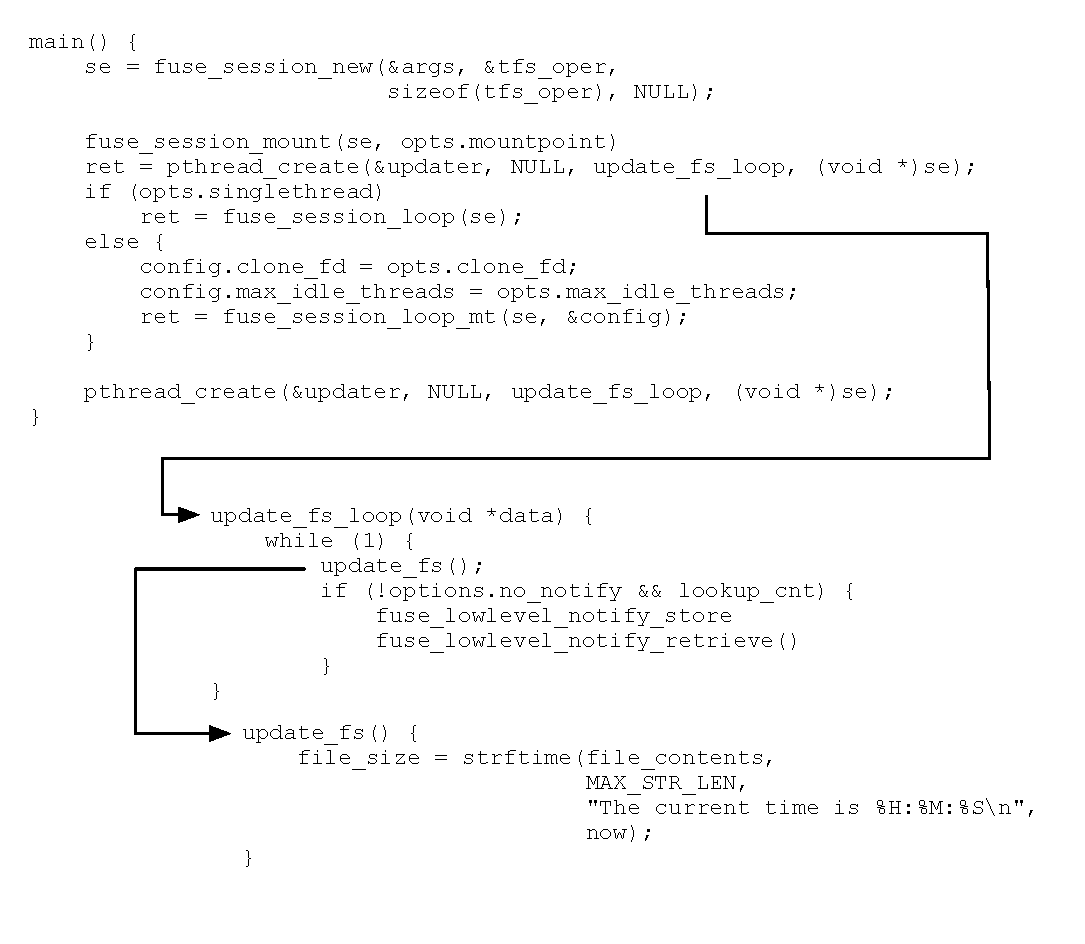
\includegraphics[scale=0.6]{figures/tfs-fuse.pdf}
	\centering
	\caption{Updating the time in the TFS file "\cf{file\_contents}"}
	\label{fig:tfs-fuse}
\end{figure}

Depending on whether the filesystem is single-threaded or multi-threaded it will then call one of the following functions:

\begin{itemize}
	\item \cf{fuse\_session\_loop()} -- Enter a single threaded event loop
	\item \cf{fuse\_session\_loop\_mt()} -- Enter a multi-threaded event loop
\end{itemize}

\noindent
There are two circumstances under which the event loop terminates. Either the filesystem is unmounted or the connection is explicitly severed by writing 1 to the FUSE abort file in \cf{/sys/fs/fuse/connections/NNN}. 

When the event loop terminates because the connection to the FUSE kernel module has been closed, this function returns zero and TFS will call \cf{fuse\_session\_unmount()} to unmount the filesystem if it is still mounted. The session is then destroyed. 

%%%%%%%%%%%%%%%%%%%%%%%%%%%%%%%%%%%%%%%%%%%%%%%%%%%%%%%%%%%%%%%%

\subsection{Updating the Kernel Inode Buffers}

There is a global variable called \cf{lookup\_cnt} which is initially set to 0. It is incremented during \cf{tfs\_lookup()} and decremented during \cf{tfs\_forget()}. You can see in figure \ref{fig:tfs-fuse} that the TFS thread will update the kernel's buffers associated with this inode by making a call to \cf{fuse\_lowlevel\_notify\_store()} and checking the result by calling \cf{fuse\_lowlevel\_notify\_retrieve()}. This allows processes to see new file contents (new time).

\textbf{XXX - what are these kernel buffers? need to look at that really good implementation guide ... if i can find it} 

% https://georgesims21.github.io/posts/fuse/ - splicing ... xxx come back later

\begin{lstlisting}
fuse_lowlevel_notify_retrieve()

Retrieve data from the kernel buffers

Retrieve data in the kernel buffers belonging to the given 
inode. If successful then the retrieve_reply() method will 
be called with the returned data.
\end{lstlisting}

%%%%%%%%%%%%%%%%%%%%%%%%%%%%%%%%%%%%%%%%%%%%%%%%%%%%%%%%%%%%%%%%

\subsection{TFS Operations}

There are seven FUSE operations that TFS provides which will be described below. Relevant sections of the code have been copied here but see the full source code for error checking and so on.

\bigskip
\noindent
\textbf{\cf{tfs\_lookup()}}
\bigskip

\noindent
The TFS lookup function returns information about \cf{file\_contents}  assuming this is the file being looked up otherwise an error is returned. The most interesting aspect of the function is incrementing \cf{lookup\_cnt} which is checked inside \cf{update\_fs\_loop()}. If it's set, a call is made into FUSE to inform it to synchronously store data in the kernel buffers belonging to the given inode. The stored data is marked up-to-date (no read will be performed against it, unless it's invalidated or evicted from the cache).

\begin{lstlisting}
tfs_lookup:
{
    if (strcmp(name, FILE_NAME) == 0) {
        e.ino = FILE_INO;
        lookup_cnt++;
    }
    e.attr_timeout = NO_TIMEOUT;
    e.entry_timeout = NO_TIMEOUT;
    tfs_stat(e.ino, &e.attr)                       
    fuse_reply_entry(req, &e);
}
\end{lstlisting}

\noindent
\cf{tfs\_stat()} returns basic file information for the root directory or for "file\_contents" (\cf{ino == FILE\_INO}).

\bigskip
\noindent
\textbf{\cf{tfs\_getattr()}}
\bigskip

\noindent
This function is called in response to \cf{stat(2)} and friends to return file attributes for the specified inode. 

\begin{lstlisting}
tfs_getattr(fuse_req_t req, fuse_ino_t ino,
            struct fuse_file_info *fi) 
{
    struct stat stbuf;
            
    memset(&stbuf, 0, sizeof(stbuf));
    tfs_stat(ino, &stbuf);
    fuse_reply_attr(req, &stbuf, NO_TIMEOUT);
}
\end{lstlisting}

\noindent
\cf{tfs\_stat()} is very simple returns a small number of attributes for the root directory or for "\cf{file\_contents}" as follows:

\begin{lstlisting}
    stbuf->st_ino = ino;
    if (ino == FUSE_ROOT_ID) {
        stbuf->st_mode = S_IFDIR | 0755;
        stbuf->st_nlink = 1;
    } else if (ino == FILE_INO) {
        stbuf->st_mode = S_IFREG | 0444;
        stbuf->st_nlink = 1;
        stbuf->st_size = file_size;
    }
\end{lstlisting}

\noindent
Notice that for the root directory \cf{st\_nlink} is set to 1 and not 2 as for most filesystems. \textbf{XXX---run this and show what it looks like}.

\bigskip
\noindent
\textbf{\cf{tfs\_readdir()}}
\bigskip

\noindent
Reading a directory is very simple in TFS since only information about "\cf{file\_contents}" needs to be returned.

\begin{lstlisting}
static void tfs_readdir(fuse_req_t req, fuse_ino_t ino, 
                        size_t size, off_t off, 
                        struct fuse_file_info *fi) 
{
        struct dirbuf b;

        memset(&b, 0, sizeof(b));
        dirbuf_add(req, &b, FILE_NAME, FILE_INO);
        reply_buf_limited(req, b.p, b.size, off, size);
        free(b.p);
}
\end{lstlisting}

\noindent 
As with \cf{tfs\_read()} a check is made to validate the offset. \textbf{XXX---need to do better at describing}

\bigskip
\noindent
\textbf{\cf{tfs\_open()}}
\bigskip

\noindent
There is only one thing to do for opening a file:

\begin{lstlisting}
tfs_open(fuse_req_t req, fuse_ino_t ino,
         struct fuse_file_info *fi)
{
    fi->keep_cache = 1;
    fuse_reply_open(req, fi);
}
\end{lstlisting}

\noindent
By default, fuse invalidates the page cache for an inode on every file open. Since TFS is a read-only filesystem this makes no sense. Setting \cf{keep\_cache} tells the kernel that any cached data for this file does not need to be invalidated. Other than that, there is little for \cf{tfs\_open()} to do.

\bigskip
\noindent
\textbf{\cf{tfs\_read()}}
\bigskip

\noindent
There is little for \cf{tfs\_read()} to do other than assert that \cf{ino} is equal to \cf{FILE\_INO} and then return the contents of the file. A check is made inside \cf{reply\_buf\_limited()} to see if the offset is valid and then a call is made to \cf{fuse\_reply\_buf()}.

\begin{lstlisting}
tfs_read(fuse_req_t req, fuse_ino_t ino, size_t size,
                     off_t off, struct fuse_file_info *fi
{            
    reply_buf_limited(req, file_contents, file_size, off, size);
}

static int
reply_buf_limited(fuse_req_t req, const char *buf, 
                  size_t bufsize,
                  off_t off, size_t maxsize) 
{
    if (off < bufsize)
        return fuse_reply_buf(req, buf + off,
                              min(bufsize - off, maxsize));
    else
        return fuse_reply_buf(req, NULL, 0);
}   
\end{lstlisting}

\noindent
If \cf{offset == 0} then the whole string in \cf{file\_contents} will be returned. The \cf{fuse\_reply\_buf()} function returns the data in the file.

%%%%%%%%%%%%%%%%%%%%%%%%%%%%%%%%%%%%%%%%%%%%%%%%%%%%%%%%%%%%%%%%

\subsection{Low-level FUSE Operation Definitions}

The \cf{/usr/include/fuse/fuse\_lowlevel.h} header file defines all of the operations - XXX need to figure out what to say about them. Who uses them? Any good examples?

\begin{lstlisting}
fuse_lowlevel_notify_poll() - NO 
fuse_lowlevel_notify_inval_inode() - YES (TFS)
fuse_lowlevel_notify_inval_entry() - YES (TFS)
fuse_lowlevel_notify_delete() - NO
fuse_lowlevel_notify_store() - YES (TFS)
fuse_lowlevel_notify_retrieve() - YES (TFS)
fuse_lowlevel_is_lib_option() - NO
\end{lstlisting}

\noindent
xxx

%%%%%%%%%%%%%%%%%%%%%%%%%%%%%%%%%%%%%%%%%%%%%%%%%%%%%%%%%%%%%%%%%

\section{Adding Encryption to pSPFS}

A passthrough filesystem is a fine way to explore how FUSE works but beyond that, it doesn't make for a very interesting filesystem. In this section, the filesystem will be enhanced to including encrypting regular file contents. It's also very simple XXX. The encryption key and IV (initialization vector) are hardcoded in the program. Although fine for demo purposes, this would not work in the real world. Keys and IVs should be separate from the running program. Section \ref{encryption} describes encryption and key management best practices.

The source code can be found on gitlab here:

\begin{table}[h]
\begin{tabular}{lcl}
\parbox[r]{0.5in}{
\includegraphics[scale=0.15]{figures/url.png}} & \parbox[l]{0.55in}{URL \arabic{urls} -- } & \parbox[l]{3in}{\cf{TBD---URL to go here}}
\end{tabular}
\end{table}
\stepcounter{urls}
% real URL

% https://www.highgo.ca/2019/08/08/the-difference-in-five-modes-in-the-aes-encryption-algorithm/

\noindent
\textbf{Come back here later}

I based the encryption/decryption code on a simple example that the OpenSSL Foundation have on their website that produces a standalone program which encrypts then decrypts the string "\textit{The quick brown fox jumps over the lazy dog}". You can find the program here:

\begin{table}[h]
\begin{tabular}{lcl}
\parbox[r]{0.5in}{
\includegraphics[scale=0.15]{figures/url.png}} & \parbox[l]{0.55in}{URL \arabic{urls} -- } & \parbox[l]{3in}{\cf{https://tinyurl.com/2p96usf6}}
\end{tabular}
\end{table}
\stepcounter{urls}
% https://wiki.openssl.org/index.php/EVP_Symmetric_Encryption_and_Decryption

\noindent
It's also in \cf{crypto.c} in the espfs source tree.

To get this program to work by itself, copy and paste the code snippets into \cf{crypto.c} and compile as follows:

\begin{lstlisting}
$ cc -o crypto crypto.c -lcrypto -lssl
\end{lstlisting}

\noindent
although make sure you have OpenSSL development package installed. The following command should be enough to get access to all the OpenSSL libraries and header files you need:

\begin{lstlisting}
$ [*\bfseries sudo apt install libssl-dev*]
\end{lstlisting}

\noindent
If you're interested in playing with encryption/decryption, this is a good start as you can experiment with algorithms and key sizes.

%%%%%%%%%%%%%%%%%%%%%%%%%%%%%%%%%%%%%%%%%%%%%%%%%%%%%%%%%%%%%%%%

\subsection{A Primer on Encryption}

The eSPFS filesystem will use AES symmetric encryption which is the mostly widely used algorithm for file and disk-based encryption. It will also use 256-bit keys although changing the key size is very simple for new filesystems. AES supports 128-bit, 192-bit, and 256-bit implementations, with AES 256 being the most commonly used. Intel AES-NI instructions support all three key sizes.

There are several things to point out and consider before implementing encryption support:

\begin{enumerate}
	\item AES operates on \textit{plaintext} and produces \textit{ciphertext} for encryption. It works in the opposite direction
		for decryption.
	\item AES encryption/decryption operates on 128-bit block sizes. You can't encrypt or decrypt data unit that is smaller or
		larger in a single AES operation. Thus to encrypt say a page of data, it will need to be broken down in 128-bit
		chunks. The 128-bit block size is divided into a 4x4 array containing 16 bytes. Since there are eight bits per byte, 
		the total in each block is 128 bits. The size of the encrypted data remains the same as the plaintext -- 128 bits of 
		plaintext yields 128 bits of ciphertext. This is particularly important for file encryption as we do not want to change
		the size of the file's data.
	\item Initialization Vector (IV) -- xxx. I recall interesting conversations with one government agency who wanted a unique
		IV per AES block. We just couldn't imagine how badly that would perform! 
	\item previous block vs next block re: IV
	\item To encrypt/decrypt, you always need to use the same key and IV.
	\item encryption / decryption occurs in 128-bit blocks (256 or bigger keys) therefore we need a complete block before
		we can perform an encrypt or decrypt. This may involve reading data from disk.
	\item The end of a file we may not be on a 128-bit block boundary. If this occurs there are several ways to make sure
		that we still have a 128-bit block in which to perform the encryption operation. Either we can pad the data with known
		data (zeroes for example) or can utilize a technique called "\textit{ciphertext stealing}" XXX - need to come back 
		and see what to do here - % https://en.wikipedia.org/wiki/Ciphertext_stealing - Either way we cannot increase the
		size of the file. Well we could ... explain ... CBC mode for stealing or others. explain. perhaps just add padding
		but talk about options and pros/cons
\end{enumerate}

% https://medium.com/swlh/an-introduction-to-the-advanced-encryption-standard-aes-d7b72cc8de97
\noindent
This was just a quick overview of the encryption process. There are many fine books and articles on line if you wish to learn more.

%%%%%%%%%%%%%%%%%%%%%%%%%%%%%%%%%%%%%%%%%%%%%%%%%%%%%%%%%%%%%%%%

\subsection{How The eSPFS Filesystem Works}

% an example of using CTR - https://stackoverflow.com/questions/3141860/aes-ctr-256-encryption-mode-of-operation-on-openssl
% very good doc with test vectors - https://www.ietf.org/rfc/rfc3686.txt

We need to modify each function in the \cf{fuse\_operations} structure that deals with file data. Here is our structure again. In this case we only have to modify two of the functions, namely \cf{sp\_read()} and \cf{sp\_write()} since only those functions deal with regular file data:

\begin{lstlisting}
static struct fuse_operations spfs_operations = {
    .create         = sp_create, 
    .open           = sp_open,
    .unlink           = sp_unlink,
    [*\bfseries    .read*]           [*\bfseries= sp\_read,*]
    [*\bfseries    .write*]          [*\bfseries= sp\_write,*]
    .getattr        = sp_getattr,
    .utimens        = sp_utimens,
    .readdir        = sp_readdir,
    .mkdir          = sp_mkdir,
    .rmdir          = sp_rmdir,
    .rename         = sp_rename,
    .statfs         = sp_statfs
};
\end{lstlisting}

\noindent
Note that if we were encrypting file names, we would have to modify every function since the filesystem gets passed the full path of each file on which it needs to operate.

Both read and write paths rely on two functions namely \cf{encrypt()} and \cf{decrypt()} which follow very similar paths as we'll see soon.

The encryption key and IV are hardcoded at the top of \cf{spfs.c} as follows:

\begin{lstlisting}
/* A 256-bit key */

unsigned char *key = \
    (unsigned char *)"01234567890123456789012345678901";

/* A 128-bit IV */

unsigned char *iv = (unsigned char *)"0123456789012345";
\end{lstlisting}

\noindent
Notice the comment about the fact that both of these values should not be hardcoded.

Since OpenSSL is being used for encryption, there is a specific sequence of OpenSSL operations performed in the following stages:

\begin{itemize}
	\item Setting up a context
	\item Initializing the encryption operation
	\item Providing plaintext bytes to be encrypted
	\item Finalizing the encryption operation
\end{itemize}

\noindent
During initialization we will provide an \cf{EVP\_CIPHER} object. In this case we are using \cf{EVP\_aes\_256\_cbc()}, which uses the AES algorithm with a 256-bit key in CBC mode. The code for encryption and decryption is very similar. Here is the function for encryption:

\begin{lstlisting}
 1 int
 2 encrypt(unsigned char *plaintext, int plaintext_len,
 3         unsigned char *key, unsigned char *iv,
 4         unsigned char *ciphertext)
 5 {
 6     EVP_CIPHER_CTX *ctx;
 7     int             len, ciphertext_len;
 8  
 9     ctx = EVP_CIPHER_CTX_new();
10  
11     EVP_EncryptInit_ex(ctx, EVP_aes_256_cbc(), NULL, key, iv);
12  
13     EVP_EncryptUpdate(ctx, ciphertext, &len,
14                       plaintext, plaintext_len);
15     ciphertext_len = len;
16  
17     EVP_EncryptFinal_ex(ctx, ciphertext + len, &len);
18     ciphertext_len += len;
19  
20     EVP_CIPHER_CTX_free(ctx);
21  
22     return ciphertext_len;
23 }
\end{lstlisting}

\noindent
Here are the steps taken:

\begin{itemize}
	\item line 9 -- Sets up a context
	\item line 11 -- Initializes the encryption operation
	\item line 13-14 -- Provides the plaintext bytes to be encrypted. The ciphertext is returned in \cf{ciphertext}.
	\item line 17 -- Finalize the encryption operation
\end{itemize}

\noindent
XXX --- shouldn't get a different size back. Need to do some research here.

The \cf{decrypt()} function is very similar. Differences are highlighted in bold but you will still see the same sequence of steps:

\begin{lstlisting}
 1 int
 2 decrypt(char *ciphertext, int ciphertext_len, unsigned char *key,
 3         unsigned char *iv, char *plaintext)
 4 {
 5     EVP_CIPHER_CTX *ctx;
 6     int len, plaintext_len;
 7  
 8     ctx = EVP_CIPHER_CTX_new();
 9  
10     [*\bfseries EVP\_DecryptInit\_ex(ctx, EVP\_aes\_256\_cbc(), NULL, key, iv);*]
11  
12     [*\bfseries EVP\_DecryptUpdate(ctx, (unsigned char *)plaintext,*]
13                      [*\bfseries \&len, (unsigned char *)ciphertext,*]
14                      [*\bfseries ciphertext\_len)) {*]
15  
16     plaintext_len = len;
17  
18     EVP_DecryptFinal_ex(ctx, plaintext + len, &len);
19  
20     plaintext_len += len;
21  
22     EVP_CIPHER_CTX_free(ctx);
23 
24     return plaintext_len;
25 }
\end{lstlisting}

\noindent
This is the easy part. If we could simply call \cf{encrypt()} from within \cf{sp\_write()} as follows:

\textbf{XXX---NO! Can't do strlen(). It might not be text. Use "size"}

\begin{lstlisting}
sp_write(const char *path, const char *buf, size_t size, 
         off_t offset, struct fuse_file_info *fi)
{
    char    *ciphertext, *plaintext = (char *)buf;
    ...    
    ciphertext = (char *)malloc(size);
    encrypt(plaintext, strlen(plaintext), key, iv, ciphertext);
    pwrite(fd, ciphertext, size, offset);
    free(ciphertext);
    ...
}
\end{lstlisting}

\noindent
we would be done. Just simply allocate a buffer the same size as \cf{buf}, encrypt the data and write it out to disk. In fact, this is how I started and it works to some degree. Similarly for \cf{sp\_read()} / \cf{decrypt()}. But problems arise very quickly. Just try copying in our \cf{lorem-ipsum} file:

\begin{lstlisting}
$ [*\bfseries ls -l lorem-ipsum*]
-rw-r--r-- 1 spate spate 2972 Dec  4 15:43 lorem-ipsum
\end{lstlisting}

\noindent
The file is 2972 bytes and recall that the AES block size is 128-bits (16 bytes). This means that there are 12 bytes at the end of the file. XXX padding is used so 2972 bytes are written but when reading the file back we only get 2960 as the length returned from \cf{decrypt()}. 

We could pad the last block but that would result on the ciphertext being longer than the plaintext. We certainly don't want to write extra ciphertext to disk so we utilize a technique called \textit{ciphertext stealing}. 

There is a NIST special publication that covers ciperhtext stealing namely \textit{Recommendation for Block Cipher Modes of Operation: Three Variants of Ciphertext Stealing for CBC Mode}. 

\begin{table}[h]
\begin{tabular}{lcl}
\parbox[r]{0.5in}{
\includegraphics[scale=0.15]{figures/url.png}} & \parbox[l]{0.55in}{URL \arabic{urls} -- } & \parbox[l]{3in}{\cf{https://tinyurl.com/37nd7x6v}}
\end{tabular}
\end{table}
\stepcounter{urls}
% https://nvlpubs.nist.gov/nistpubs/legacy/sp/nistspecialpublication800-38a-add.pdf

\noindent
NIST special publications will be covered in more detail in chapter \ref{security}. The mathematics is quite intense so you may be better off viewing  the Wikipedia page.

Need a figure here 

we will do CBC-CS1 or CS2???

C example - % https://github.com/BrianGladman/aes/blob/master/aesxam.c
another description - % https://stackoverflow.com/questions/49494793/cbc-cipher-text-stealing-decryption
video - % https://www.youtube.com/watch?v=PkSWFahIRzw

Here is the algorithm that is being followed for the write path

\begin{lstlisting}
sp_write(buf, size, ...)
{
    if amount is divisible by 128? {
        call encrypt_decrypt()
        write data
    } else {
        if we are in the middle of the file {
             read in more data to make everything 128-bit divisible
             call encrypt_decrypt()
             write data
        } else {
             steal
             call encrypt_decrypt()
             write data
        }
    }  
}
\end{lstlisting}

\noindent
Need to understand various reads/writes in the middle of the file.

Reading is a little easier XXX or is it?

\begin{lstlisting}
sp_read(buf, size, ...)
{
    if amount is divisible by 128? {
        call encrypt_decrypt()
        write data
    } else {
        if we are in the middle of the file {
             read in more data to make everything 128-bit divisible
             call encrypt_decrypt()
             write data
        } else {
             steal
             call encrypt_decrypt()
             write data
        }
    }  
}
\end{lstlisting}

\noindent
xxx

%%%%%%%%%%%%%%%%%%%%%%%%%%%%%%%%%%%%%%%%%%%%%%%%%%%%%%%%%%%%%%%%

\subsection{Extending eSPFS}

There are several things that can be done to enhance eSPFS. First of all, embedding encryption keys in the program is not a secure way to provide encryption. One enhancement would be to provide a password for the encryption key that is entered on the command line when starting the FUSE program. You should take a look at PBKDF2 (Password-Based Key Derivation Function 2) which is a key derivation function.

Another possible enhancement would be to utilize the OpenSSL AES-NI engine so that all encryption/decryption uses the Intel AES-NI hardware instructions. It's very likely that these instructions are available on your system but to find out for sure, run the following command:

\begin{lstlisting}
$ [*\bfseries grep -m1 -o aes /proc/cpuinfo*]
aes
\end{lstlisting}

\noindent
and check to see that \cf{aes} is displayed

% https://stackoverflow.com/questions/25284119/how-can-i-check-if-openssl-is-support-use-the-intel-aes-ni - gives a way to compare with/without although on my VMs, the results are the same. Maybe come back to this. Ah, but this sets an option for Intel architectures

\textbf{An additional enhancement --- xxx cache info so that we don't set up and EVP stuff every time}

%%%%%%%%%%%%%%%%%%%%%%%%%%%%%%%%%%%%%%%%%%%%%%%%%%%%%%%%%%%%

\section{FUSE Performance}

TBD

Although the performance of FUSE can be an issue in many production environments, the simplicity of providing a FUSE-based file system without dealing with kernel releases and symbol versioning can be a big win for both foul system, vendors, and customers. For example, when I was a Thales, we needed to provide a new version of the kernel based filesystem. Every time there was a kernel update. This was a substantial headache for both Thales and the customer base. We also had a FUSE-based encryption file system that avoided many of these headaches and then several examples any performance of a head that's a filesystem hat well, not an issue in specific custom environments.

% https://dl.acm.org/doi/fullHtml/10.1145/3310148 - looks good on performance

XXX need to explain - context switches etc. copying data > 2 times ...

good article here - %https://dl.acm.org/doi/fullHtml/10.1145/3310148
% https://www.usenix.org/sites/default/files/conference/protected-files/atc19_slides_bijlani.pdf
more architecture perhaps % https://arxiv.org/pdf/1403.5976.pdf
% https://www.fsl.cs.stonybrook.edu/docs/fuse/fuse-performance-fast17.pdf
see FUSE\_ CAP - capabilities - % https://www.cs.hmc.edu/~geoff/classes/hmc.cs135.201109/homework/fuse/fuse_doc.html 

%%%%%%%%%%%%%%%%%%%%%%%%%%%%%%%%%%%%%%%%%%%%%%%%%%%%%%%%%%%%%%%%

\subsection{Improving Performance with eBPF}\label{fuse-ebpf}

eBPF has been covered several times in the book and is seen as offering many new capabilities to the Linux kernel going forwards. One additional area of interest is in improving FUSE performance. 

Ashish Bijlani, and Umakishore Ramachandran who are at Georgia Institute of Technology have been working on some FUSE enhancements under the umbrella of the EXTFUSE project. They presented their findings at the 2019 USENIX Annual Technical Conference

- See methodology section for some performance features - page 63

- Faster storage is worse for fuse. Page 64

- Performance - We found that for many workloads, an optimized FUSE can perform within 5\% of native Ext4. However, some workloads are unfriendly to FUSE and even if optimized, FUSE degrades their performance by up to 83\%. Also, in terms of the CPU utilization, the relative increase seen is 31\%.


% https://events19.linuxfoundation.org/wp-content/uploads/2017/11/When-eBPF-Meets-FUSE-Improving-Performance-of-User-File-Systems-Ashish-Bijlani-Georgia-Tech.pdf

The presentation can be found here:

\begin{table}[h]
\begin{tabular}{lcl}
\parbox[r]{0.5in}{
\includegraphics[scale=0.15]{figures/url.png}} & \parbox[l]{0.55in}{URL \arabic{urls} -- } & \parbox[l]{3in}{\cf{https://tinyurl.com/2p8zfv29}}
\end{tabular}
\end{table}
\stepcounter{urls}
% https://events19.linuxfoundation.org/wp-content/uploads/2017/11/When-eBPF-Meets-FUSE-Improving-Performance-of-User-File-Systems-Ashish-Bijlani-Georgia-Tech.pdf

\noindent
There is also a detailed Usenix paper 

\begin{table}[h]
\begin{tabular}{lcl}
\parbox[r]{0.5in}{
\includegraphics[scale=0.15]{figures/url.png}} & \parbox[l]{0.55in}{URL \arabic{urls} -- } & \parbox[l]{3in}{\cf{https://tinyurl.com/h8ztwwht}}
\end{tabular}
\end{table}
\stepcounter{urls}
% https://www.usenix.org/system/files/atc19-bijlani.pdf

\noindent
Work continues at Georgia Tech at the time of writing under the ExtFUSE project. Changes being looked at apply to Gluster, Ceph, EncFS, Android and SDCardFS filesystems.

The ExtFUSE feature source code can be found here:

\begin{table}[h]
\begin{tabular}{lcl}
\parbox[r]{0.5in}{
\includegraphics[scale=0.15]{figures/url.png}} & \parbox[l]{0.55in}{URL \arabic{urls} -- } & \parbox[l]{3in}{\cf{https://github.com/extfuse/extfuse}}
\end{tabular}
\end{table}
\stepcounter{urls}
% https://github.com/extfuse/extfuse

\noindent
It will be interesting to see if/when these changes are adopted. Hmm! There have been no changes since 2020. Odd!

%%%%%%%%%%%%%%%%%%%%%%%%%%%%%%%%%%%%%%%%%%%%%%%%%%%%%%%%%%%%%%%

\section{Conclusion}

This chapter covered the FUSE architecture and showed how to build user-space filesystems that increases the speed of development and ease of debugging. There has been a little written about FUSE internals, so the goal of this chapter was to document the structures and functions that make up both the FUSE kernel components, as well as the \cf{libfuse} library.

Three example filesystems were presented using both the high-level and low-level APIs. The first just passed operations through to the underlying filesystem without modification which showed how to build a FUSE-based filesystem. The second added encryption for regular file contents using AES encryption in CBC-CS2 mode, a popular encryption algorithm with widely used and NIST recommended cipher mode (\textbf{XXX---check words are correct}). The third example, taken from the \cf{libfuse} source code, showed how to use the low-level API

There have been concerns about the performance of FUSE since its inception and there have been many improvements throughout its history with some new changes coming via eBPF. For high-performance filesystem, regular disk-based filesystems will suffice but there are several use cases where the FUSE-based approach works well. When I was at Thales we actually had two encrypting filesystems, one in the kernel and one FUSE-based. Customers used both depending on their use cases. 
